%%%%%%%%%%%%%%%%%%%%%%%%%%%%%%%%%%
% Classe Principal da monografia %
%%%%%%%%%%%%%%%%%%%%%%%%%%%%%%%%%%

%\documentclass[12pt,openright,oneside,a4paper,english,brazil]{./definitions/unifil}
\documentclass[12pt,openright,oneside,a4paper,english,french,spanish,brazil]{./definitions/unifil}

% TODO - Definir título da sua monografia %
\titulo     {Analise da eficiência da implementação de componente dinâmico em algoritmos de enxame de partículas aplicados ao problema de Job Shop Flexível}
\autor      {Matheus Muriel}
\instituicao{Centro Universitário Filadélfia}
\local      {Londrina}
\data       {2021}
\preambulo  {Ciência da Computação}
\orientador {Ricardo Inacio Alvares e Silva}

\makeglossaries
\usepackage{algorithm}
\usepackage{algpseudocode}
\usepackage{minted}
\usepackage{mwe}
\usepackage{subfig}

%\usepackage[toc,page]{appendix}

\begin{document}
\frenchspacing

%%%%%%%%%%%%%%%%%%%%%%%%%%%%%%%%%%%%%%%%%%%%%%%%%%%%%%%%%%%%%%%%%%%%%%%%%%%%%%%%%%%%%%%%%%%
%%%%%%%%%%%%%%%%%%%%%%%%%%%%%%%%%%%%%%%%%%%%%%%%%%%%%%%%%%%%%%%%%%%%%%%%%%%%%%%%%%%%%%%%%%%
%%%%%%%%%%%%%%%%%%%%%%%%%%%%%%%%%%%%%%%%%%%%%%%%%%%%%%%%%%%%%%%%%%%%%%%%%%%%%%%%%%%%%%%%%%%

%%%%% Elementos pré-textuais %%%%%
\pretextual

\imprimircapa

% Folha de rosto

\makeatletter
\renewcommand{\folhaderostocontent}{
  \begin{center}
    \ABNTEXchapterfont{
      \textbf{
        \MakeTextUppercase{\imprimirautor}
      }
    }

    \vspace*{5cm}

    \begin{center}
      \ABNTEXchapterfont{
        \normalsize
        \textbf{
          \MakeTextUppercase{\imprimirtitulo}
        }
      }
    \end{center}

    \vspace*{1cm}

    \abntex@ifnotempty{\imprimirpreambulo}{%
      \hspace{.45\textwidth}
      \begin{minipage}{.5\textwidth}
        \SingleSpacing
        Trabalho de conclusão de curso apresentado ao \imprimirinstituicao~como parte dos requisitos para obtenção de graduação em \imprimirpreambulo.
        {\textnormal{\imprimirorientadorRotulo~\imprimirorientador.}}
      \end{minipage}%
    }%

    \vspace*{\fill}

    \bfseries\large{\imprimirlocal}
    \par
    \bfseries\large{\imprimirdata}

    \vspace*{1cm}
  \end{center}
}
\makeatother

\imprimirfolhaderosto
\clearpage{\pagestyle{empty}\cleardoublepage}
\begin{folhadeaprovacao}
	\begin{center}
		\ABNTEXchapterfont\textbf{\MakeTextUppercase{\imprimirautor}}

		\vspace*{2cm}

		\begin{center}
			\ABNTEXchapterfont\large\textbf{\MakeTextUppercase{\imprimirtitulo}}
		\end{center}

		\vspace*{2cm}
		Trabalho de conclusão de curso apresentado à banca examinadora do curso de \imprimirpreambulo~do \imprimirinstituicao~de \imprimirlocal~em cumprimento a requisito parcial para obtenção do título de Bacharel em \imprimirpreambulo.
		\par
		\vspace*{.5in}

		\hspace{.6\textwidth}

		\begin{minipage}{.6\textwidth}
			\begin{center}
				\MakeTextUppercase{Aprovado pela \textbf{COMISSÃO EXAMINADORA} em \imprimirlocal, \imprimirdata.}
			\end{center}
		\end{minipage}

		\vspace*{\fill}
		\assinatura{{\imprimirorientador} - Orientador}
		\assinatura{Professor 1 - Examinador} %Insira o nome dos outros examinadores
		\assinatura{Professor 2 - Examinador} 
	\end{center}
\end{folhadeaprovacao}
%\begin{epigrafe}
  \vspace*{\fill}
  \begin{flushright}
    %%
    \lipsum[1]
  \end{flushright}
\end{epigrafe}
%\begin{agradecimentos}

  %%Insira seus agradecimentos
  \lipsum[1]
  \lipsum[1]
\end{agradecimentos}  % Opcional %
%\begin{epigrafe}
  \vspace*{\fill}
  \begin{flushright}
    \textit{"Pode colocar qualquer coisa entre aspas que as pessoas vão acreditar." \\
    (Albert Einstein)}
  \end{flushright}
\end{epigrafe}        % Opcional %
%%Altere as informações do resumo%%
\noindent{
    MURIEL; MATHEUS, F. 
    \textbf{\imprimirtitulo}. 
    Trabalho de Conclusão de Curso (Graduação) - 
    \imprimirinstituicao. 
    \imprimirlocal, 
    \imprimirdata.
}
\par

\begin{resumo}
    O \textit{Flexible Job Shop Problem} (FJSP) é um complexo problema de otimização de análise combinatória pertencente à classe de problemas NP-Hard. Esse problema consiste em um cenário onde existem diversos conjuntos de tarefas, chamadas \textit{jobs}, e diversas máquinas diferentes que podem processar essa tarefa, e tem como objetivo encontrar um agendamento que execute todas as operações na menor quantidade de tempo possível. Por se tratar de um problema NP-Hard não é possível encontrar a melhor solução, então ao longo do tempo foram propostos diversos tipos de algoritmos para encontrar uma solução boa o suficiente para o problema, uma dessas abordagens são os algoritmos bio inspirados nos quais se utilizam padrões observados na natureza para resolver problemas. Um desses padrões observados na natureza é o comportamento de enxames de abelhas e o movimento migratório de bandos de aves, o comportamento desses bandos é usado como heurística no algoritmo \textit{Particle Swarm Optimization} (PSO) onde cada individuo de uma população de partículas utiliza a média entre sua melhor posição já visitada (\textit{pBest}) e a melhor posição já visitada entre todos da população (\textit{gBest}) para obter uma nova posição, assim a cada rodada a população converge para um resultado ótimo. Porém, em alguns casos o algoritmo PSO pode convergir prematuramente para um mínimo local e chegar a uma solução não ótima. Já foram propostas modificações dinâmicas no PSO para resolver o problema de FJSP, mas apenas em cenários multiobjetivo, ou seja, com mais de um critério de avaliação de qualidade. Esse trabalho foca no cenário mono objetivo e descreve a implementação, testes e resultados de uma nova abordagem, introduzindo componentes de inércia dinâmicos nas partículas e obteve resultados que demonstram uma redução de $3,90\%$ no tempo final de \textit{makespan}, de $16,63\%$ no desvio padrão e de $33,76\%$ na variância. Uma significativa melhora na confiabilidade e na chance de se obter melhores resultados na execução do algoritmo em comparação com PSO base.\vspace{\onelineskip}

%%Adicione as palavras chaves após os dois pontos '':''%%
%\noindent\textbf{Palavras-chaves}: 3 ou mais.
\noindent\textbf{Palavras-chave}: PSO; Otimização por enxame de partículas; Particle Swarm Optimization; FJSP; Flexible Job Shop Problem; Inteligência Populacional; Componentes dinâmicos.
\end{resumo}

	%%Altere as informações do resumo%%
\noindent{SOBRENOME; NOME, D. \textbf{\imprimirtitulo}. Trabalho de conclusão de curso (Graduação) - \imprimirinstituicao. \imprimirlocal, \imprimirdata.}
\par
	%%Se o seu resumo não for em inglês, altere o ``Abstract'' e ``english'' abaixo.
\begin{resumo}[Abstract]
\begin{otherlanguage*}{english}
	%%Write your abstract in foreign language here%%
\emph{
Extended abstract in English or another foreign language. 30 lines, simple spacing.
\lipsum[5]
}
\vspace{\onelineskip}
\noindent
	%%Add the keywords after the colon '':''%%
\emph{	
\textbf{Keywords}: 3 or more.
}
\end{otherlanguage*}
\end{resumo}


%%% Lista de Figuras %%%
\newpage
\pdfbookmark[0]{\listfigurename}{Lista de Figuras}
\listoffigures*
\cleardoublepage
%%% Lista de Figuras %%%

%%% Lista de Tabelas %%%
\renewcommand{\listtablename}{Lista de Tabelas}
\listoftables*
\clearpage
%%% Lista de Tabelas %%%



\newglossaryentry{pso}{
  type=\acronymtype, 
  name={PSO},
  description={Particle Swarm Optimization}, 
  first={\textit{Particle Swarm Optimization} (PSO)\glsadd{pso}}, 
  see=[Glossary:]{pso}
}
%\gls{pso}

\newglossaryentry{jsp}{
  type=\acronymtype, 
  name={JSP},
  description={Job Shop Problem}, 
  first={\textit{Job Shop Problem} (JSP)\glsadd{jsp}}, 
  see=[Glossary:]{jsp}
}

\newglossaryentry{fjsp}{
  type=\acronymtype, 
  name={FJSP},
  description={Flexible Job Shop Problem}, 
  first={\textit{Flexible Job Shop Problem} (FJSP)\glsadd{fjsp}}, 
  see=[Glossary:]{fjsp}
}

\newglossaryentry{tfjsp}{
  type=\acronymtype, 
  name={TFJSP},
  description={Total Flexible Job Shop Problem}, 
  first={Total \textit{Flexible Job Shop Problem} (TFJSP)\glsadd{tfjsp}}, 
  see=[Glossary:]{tfjsp}
}

\newglossaryentry{pfjsp}{
  type=\acronymtype, 
  name={PFJSP},
  description={Parcial Flexible Job Shop Problem}, 
  first={Parcial \textit{Flexible Job Shop Problem} (PFJSP)\glsadd{pfjsp}}, 
  see=[Glossary:]{pfjsp}
}

%\printglossary
\printglossary[title=Lista de Siglas, style=long, type=\acronymtype, nonumberlist]


\renewcommand{\listalgorithmname}{Lista de Algoritmos}
\listofalgorithms
\clearpage

\tableofcontents*
  
  \setlength\absleftindent{0cm}
  \setlength\absrightindent{0cm}
  
  %fonte do ambiente%
  \abstracttextfont{\normalfont\normalsize}

  %intentação e espaçamento entre parágrafos%
  \setlength{\absparindent}{0pt}
  \setlength{\absparsep}{18pt}

%\pdfbookmark[0]{\listfigurename}{lof}
%\listoffigures*
%\cleardoublepage
%%%%% Fim dos Elementos pré-textuais %%%%%

%%%%%%%%%%%%%%%%%%%%%%%%%%%%%%%%%%%%%%%%%%%%%%%%%%%%%%%%%%%%%%%%%%%%%%%%%%%%%%%%%%%%%%%%%%%
%%%%%%%%%%%%%%%%%%%%%%%%%%%%%%%%%%%%%%%%%%%%%%%%%%%%%%%%%%%%%%%%%%%%%%%%%%%%%%%%%%%%%%%%%%%
%%%%%%%%%%%%%%%%%%%%%%%%%%%%%%%%%%%%%%%%%%%%%%%%%%%%%%%%%%%%%%%%%%%%%%%%%%%%%%%%%%%%%%%%%%%

%%%%% Elementos Textuais %%%%%
\textual

\renewcommand{\ABNTEXchapterfont}{\fontfamily{cmr}\fontseries{b}\selectfont}
\renewcommand{\ABNTEXchapterfontsize}{\Large}

\renewcommand{\ABNTEXsectionfont}{\uppercase{\fontfamily{cmr}\fontseries{b}\selectfont}}
\renewcommand{\ABNTEXsectionfontsize}{\large}

%%%%%%%%%%%%%%%%%%%%%%%%%%%%%%%%%%%%%%%%%%%%%%%%%%%%%%%%%%%%%%%%%%%%%%%%%%%%%%%%%%%%%%%%%%%%%%%

%% 1 ::: Introdução
\chapter{Introdução}
    Em um ambiente de produção industrial moderna a optimização é um ponto de grande importância, devido à constante mudança e alta concorrência. Em ramos como a manufatura isso se mostra especialmente importante, podendo ser o fator decisório para o sucesso de uma empresa \cite{Wari2016}.\hfill  
    
    Um dos exemplos de otimização em sistemas de manufatura é dentro de um cenário onde existem diversas máquinas independentes e uma fila de tarefas não homogêneas, e o objetivo é achar uma programação de onde cada tarefa será executada e em qual ordem, de maneira a economizar o máximo de tempo e energia.\newline

    Em um ambiente de alta concorrência é importante que essa ordem seja encontrada quanto antes, pois essa demora para encontrar a solução significa perda de tempo de produção. Porém, a busca de um bom escalonamento, ou seja, a configuração e ordem de execução, não é uma tarefa fácil. Pois, o número de possibilidades de arranjos cresce exponencialmente, e computar todas as soluções possíveis torna-se inviável após alguns níveis. \newline

    Por causa dessa característica exponencial conforme o número de máquinas e o número de problemas, esse problema de escalonamento é classificado como um problema de otimização de análise combinatória e pertence à classe de problemas \textit{NP-Hard}. \newline

    Os problemas da classe \textit{NP-Hard} são aqueles onde a resposta não pode ser encontrada computacionalmente em um tempo polinomial, ou seja, em um tempo razoável, porém uma solução pode ser verificada em tempo polinomial \cite{Eswaramurthy2008}.\newline

    Existem diversos problemas clássicos de produção e manufatura enquadrados em problemas de otimização e escalonamento, o que torna esse assunto uma área de muito interesse para pesquisadores do mundo inteiro.\newline

    Dentre os problemas clássicos de escalonamento e planejamento de produção estão: 
    \textit{Single Machine Scheduling Problem}, 
    \textit{Parallel Machine Scheduling Problem}, 
    \textit{Flow Shop Scheduling Problem}, 
    \textit{Job Shop Scheduling Problem} e 
    \textit{Open Shop Scheduling Problem} 
    \cite{Allahverdi2008}.\newline

    Como esses problemas não são possíveis de serem resolvidos em tempo polinomial, não é possível encontrar uma solução perfeita para eles. Mas é possível encontrarmos uma solução boa o suficiente, conforme os critérios de avaliação do problema, essa solução é chamada solução ótima.\newline

    \textit{Job Shop Scheduling Problem} (JSSP) é um do problema pertencente a classe de problemas \textit{NP-Hard}, ele chama muito a atenção de pesquisadores por ser um problema com diversas aplicações no mundo real, seja em ambientes de manufatura ou em planejamento de produção, ou até mesmo em logística \cite{Cheng1996}.\newline

    Nesse problema, temos um conjunto $m$ de máquinas e um conjunto $n$ de tarefas chamadas \textit{jobs}, sendo cada \textit{job} uma sequência de operações, cada uma com seu determinado tempo de execução. \newline 

    O objetivo é encontrar um escalonamento que combine todas as máquinas de forma que minimize a quantidade de tempo ocioso de cada máquina, assim atingindo o objetivo de forma que seja mais econômica e eficiente \cite{Cheng1996}. \newline

    O problema de JSP é comprovadamente pertencente à classe \textit{NP-Hard} quando em um ambiente com duas ou mais máquinas, como demonstrado por \cite{Lenstra1979}. \newline

    Porém, assim como visto por \cite{Bagchi1999} existem algumas restrições no cenário de JSP, dentre elas:
    \begin{itemize}
        \item Duas operações do mesmo \textit{job} não podem ser executadas em simultâneo;
        \item Nenhuma máquina pode executar simultaneamente mais de uma operação;
        \item As restrições e configurações de processamento são conhecidas previamente e não são alteradas;
        \item Todo \textit{job} deve ser processado até o fim, mas é permitido que haja pausas e esperas entre suas operações;
        \item As máquinas são homogêneas;
        \item Nenhum \textit{job} pode ser processado duas vezes na mesma máquina;
        \item As operações são atômicas, não sendo possível interromper ou pausar a execução da mesma;
    \end{itemize}

    O problema de Job Shop Flexível ou \textit{Flexible Job Shop Problem} (FJSP) é uma extensão do JSP onde é possível que uma operação seja executada em mais de uma máquina. Sendo assim deve se além de determinar a ordem e o local de execução de cada \textit{job}, também é preciso determinada ordem e local de execução das operações. Assim sendo considerado uma extensão mais complexa do JSP \cite{Jansen2000}. \newline

    Além disso, o problema de FJSP pode ser dividido em dois tipos, o parcial (P-FJSP), onde uma operação só pode ser executada por um subconjunto de máquinas, ou o total (T-FJSP), onde qualquer operação pode ser executada por qualquer máquina. O FJSP tem as mesmas restrições do JSP exceto a que diz que nenhum \textit{job} pode ser processado duas vezes na mesma máquina. \newline

    Ao longo do tempo já foram propostas diversas abordagens para resolver o problema de FJSP, dentre elas o \textit{Branch and Bound} \cite{Nababan2008}, a 
    \textit{Integer Programming} \cite{Pan2007}, a 
    \textit{Dynamic Programming} \cite{Gromicho2012}, 
    \textit{Evolutionary Algorithm} \cite{Pezzella2008}, e até mesmo técnicas híbridas \cite{Zhang2009}, onde duas ou mais abordagens são associadas para compor um algoritmo híbrido. \newline

    Um desses algoritmos propostos é o algoritmo de Otimização por Enxame de Partículas ou \textit{Particle Swarm Optimization} (PSO) proposto por \cite{Kennedy1995} e trabalha com um grupo de indivíduos cada um tendo: direção, velocidade, a informação da sua melhor posição e a informação da melhor posição entre todos os indivíduos do grupo, e com essas informações cada indivíduo consegue tirar sua média e a cada rodada do algoritmo ir chegando mais perto do objetivo. \newline

    Outra abordagem que tem tido bons resultados em diversos problemas práticos \cite{Qing2012} são os Algoritmos Genéticos ou \textit{Genetic Algorithms} (GA), proposto por \textit{John Henry Holland} sendo inspirado na teoria da evolução de Charles Darwin, simulando a transmissão de genes dos indivíduos mais aptos por meio da simulação de operações de cruzamento e de mutações, para selecionar os indivíduos mais aptos. \newline

    Neste trabalho iremos demonstrar e comparar a eficiência de uma abordagem híbrida do Algoritmo PSO com componentes evolutivos de GA, tornando assim esse algoritmo mais dinâmico, além de demonstrar sua eficiência em diferentes cenários reais de aplicação na indústria.\newline


%% 1 ::: Introdução
%% 1.1
\section{Problemas de Agendamento}
    %% Interlúdio do [Problemas de Agendamento] %%
        Problemas de agendamento estão muito presentes atualmente, e existem diretamente em diversos cenários, tais como planejamento de produção, sistemas de manufatura, sistemas de produção, processamento de informação, gerenciamento de rotas de logísticas, etc. e indiretamente nos computadores através do escalonamento de processos do sistema operacional.\newline

        Com tantos possíveis cenários de aplicação é natural que existam inúmeras sub-divisões deste problema. Porém, a maioria deles tem características em comum. Geralmente eles se baseiam em um conjunto de recursos e um conjunto de demandas, e visa ordenar as execuções das demandas e as distribuir entre os recursos, isso de modo a alcançar da melhor possível um ou mais objetivos, que podem ser, por exemplo, o tempo total para o algoritmo executar o agendamento (também chamado \textit{makespan}), o tempo total de execução de todas as tarefas no agendamento encontrado (também chamado \textit{fitness}) ou a soma total do tempo de ociosidade das máquinas.\newline

        Por essa característica de buscar um melhor resultado em um objetivo os problemas de agendamento são caracterizados como problemas de optimização, que são os problemas que a solução são aquelas que trazem um melhor resultado para o objetivo. É importante ressaltar que nesses problemas de optimização a solução não necessariamente precisa a melhor possível, mas sim uma solução boa o suficiente (também chamado solução ótima).\newline

        Os problemas de agendamento multi-objetivo consideram em simultâneo, mais de um critério de avaliação, podendo ter ou não o mesmo peso, ou nível de importância, e espera se que sejam atingidos todos os objetivos. Por causa dessa diversidade de objetivos que podem muitas vezes serem conflitantes entre si, como, por exemplo, ser mais rápido e, em simultâneo, gastar a menor quantidade possível de energia.\newline

        Já os problemas de agendamento mono-objetivo lidam somente com um critério de avaliação, o que diminui significativamente a dificuldade para encontrar uma solução, porém, em contrapartida, define uma importância maior para o objetivo em questão, sendo necessário um maior nível de refinamento da solução.
    %% Fim do Interlúdio do [Problemas de Agendamento] %%

    %% 1 ::: Introdução
    %% 1.1 ::: Problemas de Agendamento
    %% 1.1.1
    \subsection{Definição}
        Como foi definido por \cite{Bagchi1999} um problema de escalonamento de tarefas computacionais (\textit{jobs}) é um problema de otimização aonde os recursos limitados são alocados no tempo de execução dos recursos, com as diferentes tarefas podendo ser executadas em paralelo entre as diversas maquinas, porém, cada atividade única sendo executada sequenciamento em uma só maquina.\newline

        Assim como a grande maioria dos problemas de origem combinatória, ou seja, que um fator depende o fator anterior, formando assim uma combinação de fatores, o problema de escalonamento é um problema da classe NP-Hard da qual não é possível se encontrar a melhor solução possível em um tempo polinomial, ou seja, computacionalmente aceitável, devido a sua quantidade de operações necessárias crescer exponencialmente, com base no tamanho do problema, tornando se assim um problema inviável de se resolver através de cálculos brutos.\newline

        Por causa disso, nesses casos de problemas NP-Hard normalmente se usam algoritmos de aproximação, que tenham um tempo de execução razoável e consigam encontrar uma solução boa o suficiente com base nos critérios de avaliação, a chamada "Solução Ótima", como visto por \cite{Lawler1993}.\newline

        Porém, esse conceito de solução ótima varia conforme o problema, em alguns casos é mais importante que essa solução seja encontrada em um tempo curto, do que ela seja alguns milissegundos mais rápida do que as outras soluções já encontradas, isso se aplica em ambientes que o agendamento deve ser feito em tempo real.\newline
        Já para um problema em que essa solução precisa ser encontrada apenas uma vez e ser replicada varias vezes, como uma estrutura de linha de montagem definitiva, vale a pena esperar algumas horas a mais se essa solução economizar tempo de produção ao longo do seu uso. Então esse critério de avaliação de solução ótima deve ser muito bem analisado de caso a caso. \newline

        Nesses ambientes de soluções aproximadas, alguns algoritmos que se destacam são os algoritmos bio inspirados, algoritmos populacionais e algoritmos evolutivos. Que conseguem simular uma inteligência biológica ou comportamentos já observados na natureza e selecionados pela evolução para encontrar uma solução ótima, de maneira similar a que um ser vivo faria.
    %% Fim do [Definição] %%


    %% 1 ::: Introdução
    %% 1.1 ::: Problemas de Agendamento
    %% 1.1.2
    \subsection{Variações}
        Diversos autores já classificaram diversas variações de problemas de escalonamento dentre eles \cite{graham1979}, \cite{Lenstra1979}, e \cite{maccarthy1993}. O que diferencia os problemas são o fluxo dos \textit{jobs} a serem processados e a capacidade dos recursos. Dentre esses problemas estão:
        \begin{itemize}
            \item \textbf{\textit{Open Shop:}} Os \textit{job} tem uma ordem de execução, porém as operações de cada \textit{job} tem uma ordem específica de execução.
            
            \item \textbf{\textit{Flow Shop:}} Os \textit{jobs} devem ser executados em um fluxo unidirecional e em uma máquina somente. E não exite uma divisão do \textit{jobs} em operações.
            
            \item \textbf{\textit{Flexible Flow Shop:}} Semelhante ao \textit{Flow Shop}, porém os \textit{jobs} podem ser divididos em operações.
            
            \item \textbf{\textit{Job Shop:}} Diferentemente do \textit{Flow Shop} o \textit{Job Shop} pode ter execuções paralelas, assim como ser dividido em operações.
            
            \item \textbf{\textit{Flexible Job Shop:}} Uma extensão do \textit{Job Shop} onde as operações de cada \textit{Job} podem ser executados em máquinas diferentes. Esse problema tem duas sub divisões, a Total, em que todas as maquinas podem executar todas as operações. E a Parcial, onde existem limitações para quais maquinas podem executar quais operações.
        \end{itemize}

        Além disso, cada um dos problemas acima podem ser sub-classificados como mono-objetivos ou multi-objetivos conforme os tipos e a quantidade de objetivos. \newline
        No caso de ter somente um único objetivo, como um menor \textit{fitness} por exemplo, ou ter mais de um objetivo, como um menor \textit{fitness} e um menor índice de inércia total.\newline

        Esse trabalho é focado no problema de \textit{Flexible Job Shop} Total, em um contexto mono-objetivo.
    %% Fim do [Problema] %%


    %% 1 ::: Introdução
    %% 1.1 ::: Problemas de Agendamento
    %% 1.1.3
    \subsection{Problema de Job Shop — JSP}
        %% Interlúdio do [Problemas de Agendamento] %%
            Como citado anteriormente o \textit{Job Shop Problem} (JSP) é um problema de escalonamento de tarefas e pertence à classe de problemas NP-Hard. Como visto por \cite{Cheng1996} o problema de \textit{Job Shop} chama muita atenção por ser um problema com diversas aplicações no mundo real, e em diversos cenários diferentes, como industria, computação e manufatura.\newline

            De acordo com \cite{Cheng1996} o problema de \textit{Job Shop} consiste em $m$ máquinas distintas e $n$ \textit{jobs} diferentes, sendo cada \textit{job} formado por diversas operações $O$ em uma ordem específica. Cada operação $Oij$ tem seu respectivo tempo de execução.\newline

            Como visto por \cite{Bagchi1999} existem algumas restrições no problema de \textit{Job Shop} dentre elas:
            \begin{itemize}
                \item Mais de uma operação de um mesmo \textit{job} não pode ser executada em simultâneo.
                \item Não existe mais de uma máquina de um mesmo tipo.
                \item As máquinas podem ficar ociosas durante o período de escalonamento.
                \item As execuções de \textit{jobs} são atômicas, ou seja, cada \textit{job} deve ser processado até o fim.
                \item Uma máquina não pode executar mais de uma operação simultaneamente.
                \item Um \textit{job} não é processado duas vezes na mesma máquina.
                \item Não é possível interromper a execução de uma operação.
            \end{itemize}
        %% Fim do Interlúdio do [Problemas de Agendamento] %%
        
        %% 1 ::: Introdução
        %% 1.1 ::: Problemas de Agendamento
        %% 1.1.3 ::: JSP
        %% 1.1.3.1
        \subsubsection{Representações}
            Para ser possível que um algoritmo encontre uma solução para o agendamento, ele precisar conhecer algumas informações, dentre elas: 
            \begin{itemize}
                \item Quantas maquinas existem;
                \item Quantos \textit{Jobs} existem;
                \item Quantas operações cada \textit{Job} possui;
                \item Em qual maquina cada operação pode ser executada;
                \item Quanto tempo cada operação leva para ser executada em sua respectiva maquina;
            \end{itemize}
        %% Fim do [Representações] %%


        %% 1 ::: Introdução
        %% 1.1 ::: Problemas de Agendamento
        %% 1.1.3 ::: JSP
        %% 1.1.3.1 ::: Representações
        %% 1.1.3.1.1
        \subsubsubsection{Instancia de um Problema}
            Na figuraX é possível ver um exemplo de uma instância de problema de \textit{Job Shop}. A onde existem duas maquinas $(M1, $ e $M2)$, dois \textit{jobs} $(J1, $ e $J2)$ e que cada \textit{job} possui duas operações $(Oj,1 $ e $Oj,2)$.\newline
            Sendo assim:\newline
            A $O1,1$ na máquina $M2$ tem o tempo de execução 9.\newline 
            A $O1,2$ na máquina $M1$ tem o tempo de execução 5.\newline
            A $O2,1$ na máquina $M1$ tem o tempo de execução 1. \newline
            A $O2,2$ na máquina $M2$ tem o tempo de execução 7. \newline

            \textit{\textbf{Inserir a figuraX aqui}}\newline
        %% Fim do [Instancia de um Problema] %%

     %%
    %% Fim do [JSP] %%


    %% 1 ::: Introdução
    %% 1.1 ::: Problemas de Agendamento
    %% 1.1.4
    \subsection{Problema de Job Shop Flexível — FJSP}
        %% Interlúdio do [FJSP]%%
            O \textit{Flexible Job Shop} é uma extensão do problema de \textit{Job Shop} em que é permitido que uma operação seja executada em mais de uma máquina. Então além de definir a ordem e a maquina de execução de cada \textit{job} também é preciso definir o agendamento das operações.\newline 
            De um lado isso traz uma maior complexidade para o algoritmo, porém possibilita uma maior número de possíveis soluções e deixa o algoritmo mais flexível para encontrar soluções. Mas por esse aumento de fatores a considerar o \textit{Flexible Job Shop} é considerado um problema mais complexo que o \textit{Job Shop}.\newline

            Existem sub divisões no problema de \textit{FJSP}, sendo elas a \textbf{Parcial} (P-FJSP) se uma operação só pode ser processada por um certo sub conjunto de máquinas, ou \textbf{Total} (T-FJSP) caso uma operação possa ser processada por qualquer máquina.\newline

            Para o \textit{Flexible Job Shop} são aplicadas as mesmas restrições do \textit{Job Shop} com exceção da que diz um \textit{job} não pode ser processado duas vezes em uma mesma maquina.\newline
        %% Fim do Interlúdio do [FJSP]%%

        %% 1 ::: Introdução
        %% 1.1 ::: Problemas de Agendamento
        %% 1.1.4 ::: FJSP
        %% 1.1.4.1
        \subsubsection{Representações}
            As representações do \textit{Flexible Job Shop} são praticamente as mesma do \textit{Job Shop} com exceção da representação do problema, devido a sua natureza flexível uma representação do \textit{Flexible Job Shop} precisa definir quanto tempo cada maquina utilizaria para processar cada operação. Porém, no caso de uma problema de \textit{Flexible Job Shop} Parcial, ou seja, em que uma operação não pode ser processada por qualquer máquina, a representação não precisa definir o tempo de processamento de todas as operações para todas as maquinas, mas somente para as máquinas que podem processar aquela operação
        %% Fim do [Representações] %%


        %% 1 ::: Introdução
        %% 1.1 ::: Problemas de Agendamento
        %% 1.1.4 ::: FJSP
        %% 1.1.4.1 ::: Representações
        %% 1.1.4.1.1
        \subsubsubsection{Instancia de um Problema}
            Na TabelaX é mostrado uma instância de um problema de \textit{Flexible Job Shop} Total. Devido a sua flexibilidade a instância de problema precisa informar quanto tempo cada maquina utilizaria para executar cada operação, logo uma instância de um problema de \textit{Flexible Job Shop} é consideravelmente maior.\newline

            A representação a seguir tem um exemplo de problema com dez maquinas $(M1, M2, M3, ..., M10)$ e dez \textit{jobs} $(J1, J2, J3, ..., J10)$ e cada \textit{job} possuindo três operações $(Oj1, Oj2 e Oj3)$.\newline

            Cada índice $ji$ da Tabelax representa o tempo $Tji$ de execução de $Oji$, para cada máquina $Mk$, sendo $k = 1,... m$, onde $m$ é a quantidade de máquinas e $n$ a quantidade de jobs, ou seja, nesse exemplo $n = 10$ e $m = 10$.\newline
            Então esse problema é de tamanho 10 x 10 como visto no benchmark de \cite{Kacem2002}.\newline

            \textit{\textbf{Inserir a TabelaX aqui}}\newline
        %% Fim do [Instancia de um Problema] %%


        %% 1 ::: Introdução
        %% 1.1 ::: Problemas de Agendamento
        %% 1.1.4 ::: FJSP
        %% 1.1.4.1 ::: Representações
        %% 1.1.4.1.2
        \subsubsubsection{Solução}

            Na FiguraX é possível ver um gráfico de Gantt para uma solução para o problema representado na TabelaX, sendo um problema de \cite{Kacem2002} de tamanho 10 x 10. Nessa solução é possível se observar:
            \begin{itemize}
                \item A máquina $M1$ executa as operações $[(O1,1), (O7,1), (O2,1)]$.
                \item Cada \textit{job} utiliza no mínimo duas máquinas para ser executado, por exemplo: o $J1$ é executado nas máquinas $M1 , M3, M4$.
                \item O \textit{fitness} dessa solução é 7.
            \end{itemize}

            ...\newline

            \textit{\textbf{Inserir a TabelaX aqui}}\newline
        %% Fim do [Solução] %%


        %% 1 ::: Introdução
        %% 1.1 ::: Problemas de Agendamento
        %% 1.1.4 ::: FJSP
        %% 1.1.4.2
        \subsubsection{Cenários de Aplicação}
            O exemplo mais claro de aplicação do problema de \textit{Flexible Job Shop} é em produção industrial e em sistemas de manufatura, o que traz muito interesse econômico para boas soluções para essa categoria de problema.\newline
            Como visto por \cite{Wari2016} nos tempos modernos onde a uma grande competição e constante melhorias tecnológicas, a organização e otimização desses processos industriais se torna um gargalo a ser resolvido e pode ser um fator decisório no sucesso de uma indústria.
        %% Fim do [Cenários de Aplicação] %%
        
     %%
    %% Fim do [FJSP] %%
    
 %%
%% Fim do [Problemas de Agendamento] %%

%%%%%%%%%%%%%%%%%%%%%%%%%%%%%%%%%%%%%%%%%%%%%%%%%%%%%%%%%%%%%%%%%%%%%%%%%%%%%%%%%%%%%%%%%%%%%%%

%% 1 ::: Introdução
%% 1.2
\section{Soluções Existentes}
    %% Interlúdio %%
        Ao longo do tempo foram propostas, testadas, revisadas e aprimoradas diversas soluções para os problemas de agendamento, e como cada cenário de aplicação difere não é possível definir qual solução é a melhor, pois isso depende de caso a caso, contudo, durante o tempo varias soluções se destacaram como mais eficientes e adaptáveis a novas demandas, cenários e objetivos. \newline
        
        Um tipo de solução muito recorrente são as baseadas em comportamento biológico. Ao longo de milhões de anos a vida biológica no planeta terra evoluiu e se adaptou para encontrar o modo mais eficiente de resolver os diversos problemas que a natureza os impõe. Então observando esses comportamentos adaptativos, foram propostos diversos algoritmos como os algoritmos populacionais que simulam como populações, como, por exemplo, bandos de aves, enxames de abelhas ou colonias de formigas usam o comportamento de bando para solucionar um problema como o de encontrar alimento, ou fugir de predadores. Ou algoritmos que simulam as próprias regras de seleção natural para evoluir indivíduos de uma população para gerar e acumular mutações para achar um individuo mais adaptado e solucionar o problema, esses são os algoritmos genéticos e algoritmos evolutivos.
    %% Fim do Interlúdio %%


    %% 1 ::: Introdução
    %% 1.2 ::: Soluções Existentes
    \subsection{Algoritmos Evolutivos}
        Os Algoritmos Evolutivos são baseados no mecanismo de seleção natural observado na natureza. Então um individuo que tem alguma característica que o destaque tem maior chance de se reproduzir e transmitir essa característica para os seus descendentes.\newline
        A estrutura básica de um algoritmo evolutivo é:
        \begin{enumerate}
            \item Inicialização da população;
            \item Analise da qualidade de cada indivíduo;
            \item Seleção dos melhores indivíduos;
            \item Cruzamento desses indivíduos, de modo a gerar uma nova população;
            \item Repetição a partir do passo 2;
        \end{enumerate}
        Essa estrutura se repete até que seja atingido o critério de parada estabelecido pelo problema em questão.\newline
        Além da estrutura básica é possível melhorar um algoritmo evolutivo através de um aprendizado continuo, ou seja, em um ambiente em que tenha mudanças constantes um algoritmo evolutivo pode se adaptar e assim se auto melhorar sem a necessidade de uma intervenção do programador.
    %% Fim do [Alg EV] %%


    %% 1 ::: Introdução
    %% 1.2 ::: Soluções Existentes
    \subsection{Algoritmos Genéticos}
        Uma derivação dos algoritmos evolutivos são os algoritmos genéticos, utilizados para buscas e para otimizações, como nos problemas de escalonamento. Essa abordagem chama atenção por conseguir lidar com uma grande diversidade de soluções, o que a torna interessante especialmente em problemas de multi-objetivo como visto por \cite{Bagchi1999}.\newline
        
        Os algoritmos genéticos são com certeza a abordagem mais utilizada dentre os algoritmos evolutivos, o que algumas vezes podem gerar a impressão de que algoritmos genéticos e evolutivos são a mesma coisa, porém como o algoritmo genético lida com uma simulação de cromossomos isso o faz com que suas estruturas sejam muito mais dinâmicas, enquanto as técnicas de algoritmos evolutivos tem estruturas mais fixas.\newline
        Para ter essa dinamicidade os algoritmos genéticos trabalham com o conceito de mutações aleatórias, que podem ou não serem boas para o indivíduo, porém, por ser uma derivação dos algoritmos evolutivos o algoritmo genético conta também com os mecanismos de seleção e cruzamento da população, o que tende a selecionar apenas os indivíduos com mutações que são positivas do ponto de vista do objetivo estabelecido.
    %% Fim do [GA] %%


    %% 1 ::: Introdução
    %% 1.2 ::: Soluções Existentes
    \subsection{Algoritmos Populacionais}
        Outra abordagem dos algoritmos bioinspirados são os algoritmos populacionais, em que normalmente não se é utilizado técnicas de evolução do indivíduo específico, mas o foco é dado no comportamento da população.\newline
        Seus cenários de aplicação vão além dos algoritmos de otimização e também são utilizados em algoritmos de busca e em efeitos visuais, sendo amplamente utilizada em filmes. \newline
        
        Os algoritmos populacionais usam o conceito de inteligência de bando, onde indivíduos simples interagem entre si e com o ambiente e juntos convergem para uma solução.\newline
        A inteligência de bando pode ser vista em diversos lugares da natureza, como em colonias de formigas, enxames de abelhas, na forma de voo migratório de aves, na forma de casa de aves predatórias como águias, na organização de cardumes de peixes.\newline

        O que torna essa abordagem interessante é a sua característica decentralizada e de auto organização, o que a torna mais extensível e adaptável a cenários distribuídos. Um exemplo da utilização de algoritmos populacionais é na auto organização de drones e robôs, definidas como \textit{Swarm Robotics}. Fazendo assim com que por se algum robô tiver um defeito isso não afete a organização do grupo. \newline
        Dentre os principais algoritmos populacionais estão:
        \begin{itemize}
            \item Optimização por Colonia de Formigas (\textit{Ant Colony Optimization}) 
            \item Difusão Estocástica de Busca (\textit{Stochastic Diffusion Search})
            \item Optimização por Enxame de Partículas (\textit{Particle Swarm Optimization})
        \end{itemize}
        
        Todos eles se baseiam em como a população de indivíduos encontram juntos um objetivo. Nesse trabalho é utilizado o algoritmo de Optimização por Enxame de Partículas. 
    %% Fim do [Algoritmos Populacionais] %%

 %%
%% Fim do [Soluções Existentes] %%

%% 1 ::: Introdução
%% 1.3
\section{Particle Swarm Optimization — PSO}
    %% Interlúdio %%
        O algoritmo de Optimização por Enxame de Partículas ou PSO da sigla em inglês para (\textit{Particle Swarm Optimization}) é um algoritmo baseado nas teorias de inteligência de enxame. E diferentemente de outros algoritmos baseados em populações, como o \textit{Ant Colony Optimization} o \textit{Particle Swarm Optimization} é baseado em uma população genérica de indivíduos, embora sejam normalmente ilustrados como uma população de aves.
    %% Fim do [Interlúdio] %%


    %% 1 ::: Introdução
    %% 1.3 ::: PSO
    %% 1.3.1
    \subsection{Historia}
        O algoritmo \textit{Particle Swarm Optimization} for proposto por \cite{Kennedy1995} e desde então tem se mostrado muito promissor para a solução de diversos problemas de optimização. Por ser um algoritmo bem simples e flexível, ao longo do tempo já foram propostas varias variações para ele. \newline
        
        Porém, o \textit{Particle Swarm Optimization} já foi alvo de várias discussões na área, pois alguns autores discordam de ele ser classificada como parte dos algoritmos evolutivos, pois embora haja variações que sim, o \textit{Particle Swarm Optimization} original não implementa mecanismos de seleção, cruzamento e mutação, critérios base para os algoritmos evolutivos. \newline
        Atualmente o \textit{Particle Swarm Optimization} é classificado como parte da família dos algoritmos de \textit{Swarm Intelligence}.
    %% Fim do [Historia] %%


    %% 1 ::: Introdução
    %% 1.3 ::: PSO
    %% 1.3.2
    \subsection{Definição}
        A definição básica do algoritmo \textit{Particle Swarm Optimization} é uma população de partículas (também chamadas indivíduos), em que cada partícula tem uma velocidade e uma direção, além das informações da sua posição, qual é a qualidade de sua posição, qual foi a melhor posição na, qual ela já esteve, e acesso a um conhecimento compartilhado entre todos os indivíduos com a melhor posição em que qualquer um deles já esteve. E assim a cada rodada as partículas se movimentam com base na sua melhor posição e na melhor posição geral, e assim a cada rodada a população converge para uma solução ótima.\newline
        
        As variáveis mais importantes do PSO são justamente as melhores posições, sendo a local normalmente chamada de $pBest$ e a geral normalmente chamada de $gBest$. Elas vão ser utilizadas para obter uma média que será a nova posição da partícula. Porém, existem resistências para que a partícula mude de direção, isso acontece por meio da inércia normalmente representada por $w$ que representa a força que tende a fazer a partícula seguir a direção onde ela já está se movendo. Essa força de inércia cresce conforme o valor de velocidade da partícula, normalmente representada por $v$, ou seja, partículas com uma maior velocidade ($v$) tendem a tem uma maior inércia ($w$).\newline
        
        No pseudocodigoX é possível uma representação de um algoritmo PSO básico, esse algoritmo tem como base a formulação de \cite{martinez2009}.
        
        \textit{inserir o pseudocodigoX aqui}

        Na definição base do algoritmo não existe uma especificação de uma fórmula para o cálculo da movimentação da partícula. Porém, na formulaX é possível ver uma representação de uma fórmula base para o cálculo de uma nova posição para a partícula.

        \textit{inserir a formulaX aqui}

     %%
    %% Fim do [Definição] %%
    

    %% 1 ::: Introdução
    %% 1.3 ::: PSO
    %% 1.3.4
    \subsection{Problemas}
        Alguns cuidados devem ser tomados para a implementação do \textit{Particle Swarm Optimization} pois o algoritmo se mal configurado através dos parâmetros de velocidade, inercia e tamanho da população, tende a convergir prematuramente para uma solução não ótima, esse problema é normalmente chamado "Convergência Prematura".\newline
        
        Algumas medidas podem ser tomadas para diminuir essa possibilidade de convergência Prematura, como valores dinâmicos de inércia e uma ponderação nos valores de importância de $pBest$ e $gBest$.
    %% Fim do [Problemas] %%


    %% 1 ::: Introdução
    %% 1.3 ::: PSO
    %% 1.3.5
    \subsection{Melhorias}
        %% Interludio %%
            Algumas técnicas podem ser usadas para melhorar o desempenho do PSO em cada cenário de aplicação. Porém, o efeito dessas abordagens varia de acordo com qual problema esta sendo resolvido e dos recursos e limitações de processamento e memoria do ambiente de processamento do algoritmo.
        %% Fim do [Interludio] %%

        \subsubsection{Multithreading}
            Uma abordagem com bons resultados é o processamento distribuído do cálculo de cada partícula como visto por \cite{Thongkrairat2019} e \cite{Kim2011}. Essa paralelização é possível graças a natureza distribuída dos algoritmos populacionais. No caso do \textit{Particle Swarm Optimization} o único fator a se considerar para uma implementação distribuída é a atualização da variavel $gBest$.\newline
            
            Um cenário que tira um bom proveito dessa abordagem são os de robôs e drones.            
        %% Fim do [Multitheading] %%

        \subsubsection{Hibridização}
            Outra melhoria que tem dado bons resultados é a hibridização de PSO com outros algoritmos, como algoritmos genéticos como demostrado por \cite{carvalho2014}, ou com outros algoritmos evolutivos.\newline
            Essas hibridizações com algoritmos evolutivos são tão boas pela característica básica do PSO de não ter componentes evolutivos em seus indivíduos, então uma adição de componentes evolutivos não atrapalha nenhum ponto do PSO. \newline
            
            Esses componentes evolutivos normalmente trabalham nos valores de inércia e de velocidade, criando partículas mais teimosas ou com uma tendência maior a fugir da convergência do grupo, o que pode ajudar a escapar de mínimos locais, evitando assim a convergência prematura.\newline
            
            Um cenário que tem um bom proveito da hibridização evolutiva do PSO são os cenários com multi-objetivo, pois os componentes de mutação de algoritmos genéticos trazem uma maior diversidade para os indivíduos da população, trazendo assim uma maior gama de exploração no espaço de soluções.
        %% Fim do [Hibridização] %%

        \subsubsection{Dinamicidade}
            Outra abordagem promissora é a implementação de componentes dinâmicos na população, ou seja, que possam mudar suas características como velocidade e inercia de maneira dinâmica, por exemplo, se uma partícula perceber que esta longe do $gBest$ e está se movendo pouco ela pode reconhecer que possivelmente esta em um mínimo local e diminuir seu valor de inércia afim ou o fator de importância do seu $pBest$.\newline
            
            Essa abordagem pode ser feita de maneira constante nas partículas, fazendo elas se atualizarem em tempo real.
        %% Fim do [Dinamicidade] %%
     %
    %% Fim do [Melhorias] %%

 %
%% Fim do [PSO] %%


\chapter{Fundamentação}
(...)

%% 1 ::: Introdução
%% 1.1
\section{Problemas de Agendamento}
%% Interlúdio do [Problemas de Agendamento] %%
Problemas de agendamento são muito comuns atualmente, pois estão diretamente presentes em diversos cenários, tais como planejamento de produção, sistemas de manufatura, linhas de montagem, processamento de informação, planejamento e gerenciamento de rotas logísticas e mesmo que de maneira indireta, também estão presentes nos computadores através de escalonadores de processos do sistema operacional.
%
Com tantos possíveis cenários de aplicação é esperado que existam diversas variações deste problema, cada uma em seu cenário, e com suas peculiaridades. Porém, a maioria destes problemas tem características em comum. Geralmente eles se baseiam em um conjunto de recursos e um conjunto de demandas, e tem como objetivo organizar as execuções dessas demandas e distribuí-las entre os recursos, de modo a alcançar da melhor maneira possível um ou mais objetivos, que podem ser, por exemplo: 
\begin{itemize}
    \item O tempo total para o algoritmo executar o algoritmo e encontrar uma solução, ou seja, um agendamento.
    \item O tempo total decorrido entre o a primeira e a ultima tarefa do agendamento (também chamado \textit{fitness} ou \textit{makespan}).
    \item Ou a soma total do tempo de ociosidade das máquinas durante o período do agendamento.\\
\end{itemize}

Devido a esta característica de buscar um melhor resultado para atender a um objetivo os problemas de agendamento são caracterizados como problemas de otimização, que são problemas nos quais o objetivo é encontrar uma solução que melhor atenda os critérios de avaliação do problema em questão.\\
%
\indent Os problemas de otimização são caracterizados por terem um numero muito grande de soluções possíveis (algumas vezes tendendo ao infinito), o que torna inviável a computação de todas essas possibilidade. Por causa dessa característica um algoritmo de otimização não necessariamente precisa encontrar a melhor solução possível entre todas as possibilidades, mas sim uma solução boa o suficiente (também chamado solução ótima) de acordo com os critérios de avaliação do problema.\\
%
Os problemas de otimização podem ser classificados em dois tipos, sendo eles: Problemas "mono-objetivos", e problemas "multi-objetivos".\\
%
Os problemas do tipo multi-objetivo consideram simultaneamente, mais de um critério de avaliação, podendo ter ou não o mesmo peso (nível de importância), e espera se que sejam atingidos de forma satisfatória todos os critérios de avaliação. Por causa dessa diversidade de objetivos que podem muitas vezes ser conflitantes entre si, como por exemplo: Ser mais rápido e gastar a menos energia.\\
%
Já os problemas to tipos mono-objetivo lidam somente com um critério de avaliação, o que diminui significativamente a dificuldade para encontrar uma solução, porém, em contrapartida, espera se um resultado melhor para o objetivo em questão, sendo necessário um maior nível de refinamento da solução.
%% Fim do Interlúdio do [Problemas de Agendamento] %%

%% 1 ::: Introdução
%% 1.1 ::: Problemas de Agendamento
%% 1.1.1
%\subsection{Definição}
Como foi definido por \cite{Bagchi1999} um problema de agendamento (também chamado de problema de escalonamento) é um problema de otimização aonde 
diversas tarefas (chamadas de \textit{jobs}) são alocados em uma ordem sequencial entre os recursos (máquinas), 
com diferentes tarefas podendo ser executadas simultaneamente
em maquinas diferentes, porém cada atividade devendo ser executada somente em uma maquina por vez, como demonstrado na
\hyperref[fig:ex-problema-escalonamento]{Figura \ref{fig:ex-problema-escalonamento}}.\\

\begin{figure}[ht]
    \centering
    \caption{Demonstração de um problema de escalonamento}
    \label{fig:ex-problema-escalonamento}
    \small{Incluir um exemplo de problema de escalonamento aqui}
\end{figure}

Assim como a grande maioria dos problemas de origem combinatória, ou seja, cujo um valor dependa do valor anterior, formando assim uma combinação de fatores, o problema de escalonamento pertence a classe de problemas NP-Hard na qual não é possível se encontrar a melhor solução em um tempo polinomial, ou seja, um tempo computacionalmente aceitável.\\

Isso acontece devido a quantidade de operações necessárias para verificar todas as possibilidades de soluções para o problema em questão, crescerem de forma exponencial com base no tamanho do problema, 
como demonstrado na \hyperref[fig:problema-exponencial]{Figura \ref{fig:problema-exponencial}},
o que torna os problemas dessa classe inviáveis de serem resolvidos através de métodos comuns de cálculos.\hfill

\begin{figure}[h]
    \centering
    \small{Incluir a representação de um problema exponencial aqui}
    \caption{Demonstração de um problema exponencial}
    \label{fig:problema-exponencial}
\end{figure}


Por causa disso, nos casos de problemas NP-Hard normalmente são utilizados algoritmos de aproximação, que tenham um tempo de execução razoável e que consigam encontrar uma solução boa o suficiente, a chamada "Solução Ótima",  com base nos critérios de avaliação do problema, como visto por \cite{lawler1993}.\\

Porém, esse conceito de solução ótima varia conforme o problema, em alguns casos é mais importante que a solução seja encontrada em um curto espaço de tempo, do que seja alguns milissegundos mais rápida do que as outras soluções já encontradas pelo algoritmo, isso se aplica por exemplo em ambientes em que o agendamento deva ser feito em tempo real.\\

Já em um cenário no qual essa solução precisa ser encontrada apenas uma vez no dia e depois ser aplicada varias vezes, como em uma estrutura de linha de montagem, vale a pena esperar algumas minutos a mais se essa solução economizar tempo de produção (e consequentemente dinheiro) ao longo de seu uso. Então esse critério de avaliação que define uma solução ótima deve ser muito bem analisado de caso a caso.\\

Nesses ambientes de soluções aproximadas, alguns algoritmos que se destacam são os algoritmos bio inspirados como: Algoritmos Populacionais e Algoritmos Evolutivos. 
Que consistem em simular uma inteligência biológica ou comportamentos já observados na natureza e selecionados pela evolução, para encontrar uma solução ótima para o problema em questão, de maneira similar a qual um ser vivo faria.\\
%% Fim do [Definição] %%


%% 1 ::: Introdução
%% 1.1 ::: Problemas de Agendamento
%% 1.1.2
%\subsection{Variações}
Vários autores já classificaram diversas variações de problemas de escalonamento, dentre eles: \cite{graham1979}, \cite{Lenstra1979}, e \cite{maccarthy1993}. E o que diferencia esses problemas é o fluxo dos \textit{jobs} a serem processados e a capacidade dos recursos.\\

\noindent Dentre esses problemas estão:
\begin{itemize}
    \item \textbf{\textit{Open Shop:}} Os \textit{job} não tem uma ordem de execução, porém as operações de cada \textit{job} tem uma ordem específica de execução.
    
    \item \textbf{\textit{Flow Shop:}} Os \textit{jobs} devem ser executados em um fluxo unidirecional e em somente uma máquina. E não exite uma divisão do um \textit{job} em operações.
    
    \item \textbf{\textit{Flexible Flow Shop:}} Semelhante ao \textit{Flow Shop}, porém os \textit{jobs} podem ser divididos em operações.
    
    \item \textbf{\textit{Job Shop:}} Diferentemente do \textit{Flow Shop} o \textit{Job Shop} pode ter execuções paralelas, assim como ser dividido em operações.
    
    \item \textbf{\textit{Flexible Job Shop:}} Uma extensão do \textit{Job Shop} onde as operações de cada \textit{job} podem ser executados em máquinas diferentes. Esse problema tem duas sub divisões, 
    \subitem \textbf{\textit{Flexible Job Shop Total}}: Na qual todas as maquinas podem executar todas as operações. 
    \subitem \textbf{\textit{Flexible Job Shop Parcial}}: Na qual existem limitações para quais maquinas podem executar quais operações.
\end{itemize}

Além disso, cada um dos problemas acima podem ser classificado em mono-objetivos ou multi-objetivos. Esse trabalho é focado no problema \textbf{\textit{Flexible Job Shop Total}}, com um contexto mono-objetivo.\\
%% Fim do [Problema] %%


%% 1 ::: Introdução
%% 1.1 ::: Problemas de Agendamento
%% 1.1.3
\subsection{Problema de Job Shop — JSP}
%% Interlúdio do [Problemas de Agendamento] %%
Como citado anteriormente o \textit{Job Shop Problem} (também chamado de JSP) é um problema de escalonamento de tarefas pertencente à classe de problemas NP-Hard. Como visto por \cite{Cheng1996} o problema de \textit{Job Shop} desperta muito interesse de pesquisadores por ser um problema com diversas aplicações no mundo real, e em vários cenários diferentes, como industria, computação e manufatura.\\

De acordo com \cite{Cheng1996} o problema de \textit{Job Shop} consiste em $m$ máquinas distintas e $n$ \textit{jobs} diferentes entre si, sendo cada \textit{job} formado por diversas operações $O$ em uma ordem específica, e cada operação $O_{ij}$ tem seu respectivo tempo de execução.\\

\noindent Como visto por \cite{Bagchi1999} existem algumas restrições no problema de \textit{Job Shop} dentre elas estão:
\begin{itemize}
    \item Não é possível executar simultaneamente duas operações de um mesmo \textit{job}.
    \item Não existe mais de uma máquina de um mesmo tipo.
    \item As máquinas podem ficar ociosas durante o período de escalonamento.
    \item As execuções de um \textit{job} são atômicas e não podem ser interrompidas.
    \item Uma máquina não pode executar mais de uma operação simultaneamente.
    \item Um \textit{job} não é processado duas vezes na mesma máquina.
    \item Não é possível interromper a execução de uma operação.
\end{itemize}
%% Fim do Interlúdio do [Problemas de Agendamento] %%
        
%% 1 ::: Introdução
%% 1.1 ::: Problemas de Agendamento
%% 1.1.3 ::: JSP
%% 1.1.3.1
%\subsubsection{Representações}
Para ser possível que um algoritmo encontre uma solução para o agendamento, ele precisar conhecer algumas informações, dentre elas: 
\begin{itemize}
    \item Quantas maquinas existem;
    \item Quantos \textit{jobs} existem;
    \item Quantas operações cada \textit{job} possui;
    \item Em qual maquina cada operação pode ser executada;
    \item Quanto tempo cada operação leva para ser executada em sua respectiva maquina;
\end{itemize}
%% Fim do [Representações] %%


%% 1 ::: Introdução
%% 1.1 ::: Problemas de Agendamento
%% 1.1.3 ::: JSP
%% 1.1.3.1 ::: Representações
%% 1.1.3.1.1
%\subsubsubsection{Instancia de um Problema}
Na 
\hyperref[fig:ex-instancia-problema-JSP]{Tabela \ref{fig:ex-instancia-problema-JSP}}
é possível ver um exemplo de uma instância de problema de \textit{Job Shop}. 
A onde existem duas maquinas $M_1, $ e $M_2$, 
dois \textit{jobs} $J_1, $ e $J_2$ 
e que cada \textit{job} possui 
duas operações $O_{j,1} $ e $O_{j,2}$.
            
\begin{table}[htb]
    \centering
    \caption{Exemplo de instancia de um problema \textit{Job Shop Problem}}
    \label{fig:ex-instancia-problema-JSP}
    \begin{tabular}[t]{lcccc}
        \hline
        &\multicolumn{2}{c}{Operação 1}&\multicolumn{2}{c}{Operação 2}\\
        $Job$&Máquina&Tempo&Máquina&Tempo\\
        \hline
        $J_1$&$M_2$&9&$M_1$&5\\
        $J_1$&$M_1$&1&$M_2$&7\\
        \hline
    \end{tabular}
\end{table}

\noindent Sendo assim:\hfill
\begin{itemize}
    \item A operação $O_{1,1}$ na máquina $M_2$ tem o tempo de execução $9$
    \item A operação $O_{1,2}$ na máquina $M_1$ tem o tempo de execução $5$
    \item A operação $O_{2,1}$ na máquina $M_1$ tem o tempo de execução $1$
    \item A operação $O_{2,2}$ na máquina $M_2$ tem o tempo de execução $7$
\end{itemize}
%% Fim do [Instancia de um Problema] %%
%% Fim do [JSP] %%


%% 1 ::: Introdução
%% 1.1 ::: Problemas de Agendamento
%% 1.1.4
\subsection{Problema de Job Shop Flexível — FJSP}
%% Interlúdio do [FJSP]%%
O \textit{Flexible Job Shop} é uma extensão do problema de \textit{Job Shop} na qual é permitido que uma operação seja executada em mais de uma máquina. Então no momento de definir a ordem e a maquina de execução de cada \textit{job} as possibilidades de arranjo são muito maiores, o que aumenta a complexidade por se tratar de um problema exponencial.\\

De um lado isso traz uma maior complexidade para o algoritmo, porém possibilita uma maior número de possíveis soluções e deixa o algoritmo mais flexível para encontrar melhores soluções. Mas por esse aumento de fatores a se considerar o \textit{Flexible Job Shop} é definido como uma extensão mais complexa do \textit{Job Shop}.\\

Como dito anteriormente, existem duas sub divisões do problema de \textit{FJSP}, sendo elas a \textbf{Parcial} (P-FJSP) se uma operação só pode ser processada por um certo sub conjunto de máquinas, ou \textbf{Total} (T-FJSP) caso uma operação possa ser processada por qualquer máquina.\\

E para ambas as sub divisões do \textit{Flexible Job Shop} são aplicadas as mesmas restrições do \textit{Job Shop} com exceção da que diz que um \textit{job} não pode ser processado duas vezes em uma mesma maquina.\hfill
%% Fim do Interlúdio do [FJSP]%%


%% 1 ::: Introdução
%% 1.1 ::: Problemas de Agendamento
%% 1.1.4 ::: FJSP
%% 1.1.4.1
%\subsubsection{Representações}
As representações do \textit{Flexible Job Shop} são praticamente as mesma do \textit{Job Shop} com exceção da representação do problema, devido a sua natureza flexível uma representação do \textit{Flexible Job Shop} precisa definir quanto tempo cada maquina utilizaria para processar cada operação.\\

Porém, no caso de uma problema de \textit{Flexible Job Shop} Parcial, ou seja, em que uma operação não pode ser processada por qualquer máquina, a representação não precisa definir o tempo de processamento de todas as operações para todas as maquinas, mas somente para as máquinas que podem processar aquela operação.\\
%% Fim do [Representações] %%


%% 1 ::: Introdução
%% 1.1 ::: Problemas de Agendamento
%% 1.1.4 ::: FJSP
%% 1.1.4.1 ::: Representações
%% 1.1.4.1.1
%\subsubsubsection{Instancia de um Problema}
Na 
\hyperref[fig:ex-instancia-problema-FJSP]{Figura \ref{fig:ex-instancia-problema-FJSP}} 
é mostrado uma instância de um problema de \textit{Flexible Job Shop} Total. De tamanho $10\times10$ retirado do benchmark de \cite{Kacem2002}.
%
Para o FJSP Total, uma instância de um problema precisa informar quanto tempo cada maquina utilizaria para executar cada operação, logo uma instância de um problema de FJSP-T é consideravelmente maior do que uma representação de problema de JSP.
%%%%%%%%%%%%%%%%%%%%%%%%%%%%%%%%%%%%%%%%%%%%%%%%%%%%%%%%%%%%%%%
\begin{table}[htb]
    \centering
    \caption{Exemplo de problema $10\times10$ de \textit{T-FJSP} de Kacem et al. 2002}
    \label{fig:ex-instancia-problema-FJSP}
    \begin{tabular}[t]{llcccccccccc}
\hline
$Job$&$O_{ji}$&$M_1$&$M_2$&$M_3$&$M_4$&$M_5$&$M_6$&$M_7$&$M_8$&$M_9$&$M_{10}$\\
\hline
\multirow{3}{*}{$J_1$}&$O_{1,1}$ & $1$ & $4$ & $6$ & $9$ & $3$ & $5$ & $2$ & $8$ & $9$ & $5$\\
&$O_{1,2}$ & $4$ & $1$ & $1$ & $3$ & $4$ & $8$ & $10$ & $4$ & $11$ & $4$\\
&$O_{1,3}$ & $3$ & $2$ & $5$ & $1$ & $5$ & $6$ & $9$ & $5$ & $10$ & $3$\\
\multirow{3}{*}{$J_2$}&$O_{2,1}$ & $2$ & $10$ & $4$ & $5$ & $9$ & $8$ & $4$ & $15$ & $8$ & $4$\\
&$O_{2,2}$ & $4$ & $8$ & $7$ & $1$ & $9$ & $6$ & $1$ & $10$ & $7$ & $1$\\
&$O_{2,3}$ & $6$ & $11$ & $2$ & $7$ & $5$ & $3$ & $5$ & $14$ & $9$ & $2$\\
\multirow{3}{*}{$J_3$}&$O_{3,1}$ & $8$ & $5$ & $8$ & $9$ & $4$ & $3$ & $5$ & $3$ & $8$ & $1$\\
&$O_{3,2}$ & $9$ & $3$ & $6$ & $1$ & $2$ & $6$ & $4$ & $1$ & $7$ & $2$\\
&$O_{3,3}$ & $7$ & $1$ & $8$ & $5$ & $4$ & $9$ & $1$ & $2$ & $3$ & $4$\\
\multirow{3}{*}{$J_4$}&$O_{4,1}$ & $5$ & $10$ & $6$ & $4$ & $9$ & $5$ & $1$ & $7$ & $1$ & $6$\\
&$O_{4,2}$ & $4$ & $2$ & $3$ & $8$ & $7$ & $4$ & $6$ & $9$ & $8$ & $4$\\
&$O_{4,3}$ & $7$ & $3$ & $12$ & $1$ & $6$ & $5$ & $8$ & $3$ & $5$ & $2$\\
\multirow{3}{*}{$J_5$}&$O_{5,1}$ & $7$ & $10$ & $4$ & $5$ & $6$ & $3$ & $5$ & $15$ & $2$ & $6$\\
&$O_{5,2}$ & $5$ & $6$ & $3$ & $9$ & $8$ & $2$ & $8$ & $6$ & $1$ & $7$\\
&$O_{5,3}$ & $6$ & $1$ & $4$ & $1$ & $10$ & $4$ & $3$ & $11$ & $13$ & $9$\\
\multirow{3}{*}{$J_6$}&$O_{6,1}$ & $8$ & $9$ & $10$ & $8$ & $4$ & $2$ & $7$ & $8$ & $3$ & $10$\\
&$O_{6,2}$ & $7$ & $3$ & $12$ & $5$ & $4$ & $3$ & $6$ & $9$ & $2$ & $15$\\
&$O_{6,3}$ & $4$ & $7$ & $3$ & $6$ & $3$ & $4$ & $1$ & $5$ & $1$ & $11$\\
\multirow{3}{*}{$J_7$}&$O_{7,1}$ & $1$ & $7$ & $8$ & $3$ & $4$ & $9$ & $4$ & $13$ & $10$ & $7$\\
&$O_{7,2}$ & $3$ & $8$ & $1$ & $2$ & $3$ & $6$ & $11$ & $2$ & $13$ & $3$\\
&$O_{7,3}$ & $5$ & $4$ & $2$ & $1$ & $2$ & $1$ & $8$ & $14$ & $5$ & $7$\\
\multirow{3}{*}{$J_8$}&$O_{8,1}$ & $5$ & $7$ & $11$ & $3$ & $2$ & $9$ & $8$ & $5$ & $12$ & $8$\\
&$O_{8,2}$ & $8$ & $3$ & $10$ & $7$ & $5$ & $13$ & $4$ & $6$ & $8$ & $4$\\
&$O_{8,3}$ & $6$ & $2$ & $13$ & $5$ & $4$ & $3$ & $5$ & $7$ & $9$ & $5$\\
\multirow{3}{*}{$J_9$}&$O_{9,1}$ & $3$ & $9$ & $1$ & $3$ & $8$ & $1$ & $6$ & $7$ & $5$ & $4$\\
&$O_{9,2}$ & $4$ & $6$ & $2$ & $5$ & $7$ & $3$ & $1$ & $9$ & $6$ & $7$\\
&$O_{9,3}$ & $8$ & $5$ & $4$ & $8$ & $6$ & $1$ & $2$ & $3$ & $10$ & $12$\\
\multirow{3}{*}{$J_{10}$}&$O_{10,1}$ & $4$ & $3$ & $1$ & $6$ & $7$ & $1$ & $2$ & $6$ & $20$ & $6$\\
&$O_{10,2}$ & $3$ & $1$ & $8$ & $1$ & $9$ & $4$ & $1$ & $4$ & $17$ & $15$\\
&$O_{10,3}$ & $9$ & $2$ & $4$ & $2$ & $3$ & $5$ & $2$ & $4$ & $10$ & $23$\\
\hline
    \end{tabular}
\end{table}
%%%%%%%%%%%%%%%%%%%%%%%%%%%%%%%%%%%%%%%%%%%%%%%%%%%%%%%%%%%%%%%
Na 
\hyperref[fig:ex-instancia-problema-FJSP]{Figura \ref{fig:ex-instancia-problema-FJSP}} 
é representado um problema com dez maquinas $(M_1, M_2, M_3, ..., M_{10})$ e dez \textit{jobs} $(J_1, J_2, J_3, ..., J_{10})$ aonde cada \textit{job} possui três operações $(O_{j1}, O_{j2}, O_{j3})$.\\
%
Cada índice $ji$ representa o tempo $T{ji}$ de execução de $O_{ji}$, para a máquina $M_k$, 
sendo $k=[1, ..., m]$, onde $m$ é a quantidade de máquinas e $n$ a quantidade de jobs, ou seja, nesse exemplo $n=10$ e $m=10$.\\
%% Fim do [Instancia de um Problema] %%


%% 1 ::: Introdução
%% 1.1 ::: Problemas de Agendamento
%% 1.1.4 ::: FJSP
%% 1.1.4.1 ::: Representações
%% 1.1.4.1.2
%\subsubsubsection{Solução}
Na 
\hyperref[fig:plot-gantt]{Figura \ref{fig:plot-gantt}} 
é possível ver um gráfico do tipo \textit{Gantt Plot} que representa uma solução para o problema representado na 
\hyperref[fig:ex-instancia-problema-FJSP]{Figura \ref{fig:ex-instancia-problema-FJSP}}, 
que é o problema de tamanho $10\times10$ do benchmark de  \cite{Kacem2002}.\\

\begin{figure}[ht]
    \centering
    \small{Incluir o grafico de gantt aqui}
    \caption{Exemplo Gráfico de Gantt}
    \label{fig:plot-gantt}
\end{figure}

\noindent Nessa solução é possível observar que:
\begin{itemize}
    \item A máquina $M_1$ executa as operações $[O_{1,1}, O_{7,1}, O_{2,1}]$.
    \item Cada \textit{job} utiliza no mínimo duas máquinas para ser executado, como por exemplo o \textit{job} $J_1$ que é executado nas máquinas $[M_1 , M_3, M_4]$.
    \item O \textit{fitness} dessa solução é $7$.
\end{itemize}
%% Fim do [Solução] %%

%% 1 ::: Introdução
%% 1.1 ::: Problemas de Agendamento
%% 1.1.4 ::: FJSP
%% 1.1.4.2
%%\subsubsection{Cenários de Aplicação}
O exemplo mais claro de aplicação do problema de \textit{Flexible Job Shop} é na produção industrial e em sistemas de manufatura, o que traz muito interesse econômico para encontrar boas soluções para essa categoria de problema.
%
Como visto por \cite{Wari2016} nos tempos modernos onde existe uma grande competição e constantes mudanças e melhorias tecnológicas, a organização e otimização desses processos industriais se torna um gargalo a ser resolvido e pode ser um fator decisório no sucesso de uma indústria.
%% Fim do [Cenários de Aplicação] %%
%% Fim do [FJSP] %%
%% Fim do [Problemas de Agendamento] %%


%%%%%%%%%%%%%%%%%%%%%%%%%%%%%%%%%%%%%%%%%%%%%%%%%%%%%%%%%%%%%%%%%%%%%%%%%%%%%%%%%%%%%%%%%%%%%%%

%% 1 ::: Introdução
%% 1.2
\section{Soluções Existentes}
%% Interlúdio %%
Ao longo do tempo foram propostas, testadas, revisadas e aprimoradas diversas soluções para os problemas de agendamento, más como cada cenário de aplicação é único, não é possível definir que uma solução é melhor do que outra, pois isso depende dos critérios de analise de cada problema, contudo, durante o tempo algumas soluções chamaram a atenção de pesquisadores, seja por serem mais eficientes ou por serem mais adaptáveis a novas demandas, cenários e objetivos.\\

Um tipo de solução muito recorrente são as soluções baseadas em comportamento biológico. 
%
Ao longo de milhões de anos a vida biológica no planeta Terra evoluiu e se adaptou para encontrar modos mais eficientes de resolver os diversos problemas que a natureza impõe. 
Então observando esses comportamentos adaptativos, foram propostos diversos algoritmos, 
como os algoritmos populacionais que simulam como populações de animais, como por exemplo, bandos de aves, enxames de abelhas ou colonias de formigas usam o comportamento de bando para solucionar um problema como o de encontrar alimento, ou fugir de predadores. 
Ou algoritmos que simulam as próprias regras de seleção natural para selecionar e evoluir indivíduos de uma população para gerar e acumular mutações afim de obter uma população de indivíduos mais adaptados e solucionar um problema, esses são os Algoritmos Genéticos e Algoritmos Evolutivos.\\
%% Fim do Interlúdio %%


%% 1 ::: Introdução
%% 1.2 ::: Soluções Existentes
%\subsection{Algoritmos Evolutivos}
Os Algoritmos Evolutivos são baseados no mecanismo de seleção natural observado na natureza e descritos por Charles Darwin. Onde um individuo que tem alguma mutação que gere uma característica positiva que o destaque dos outros indivíduos da população, tem maior chance de se reproduzir e transmitir essa característica para os seus descendentes.\\

\noindent A estrutura básica de um Algoritmo Evolutivo é:
\begin{enumerate}
    \item Inicialização da população.
    \item Analise a qualidade de cada indivíduo.
    \item Selecionar os melhores indivíduos.
    \item Cruzar esses indivíduos melhores entre si, de modo a gerar uma nova população com melhores indivíduos.
    \item Voltar e repetir a partir do passo 2.
\end{enumerate}

Essa estrutura se repete até que seja atingido o critério de parada estabelecido pelo problema em questão.\\

Além da estrutura básica é possível melhorar um Algoritmo Evolutivo através de um aprendizado continuo, ou seja, em um ambiente em que tenha mudanças constantes um Algoritmo Evolutivo pode se adaptar e assim se auto melhorar sem a necessidade de uma intervenção do programador.\\
%% Fim do [Alg EV] %%


%% 1 ::: Introdução
%% 1.2 ::: Soluções Existentes
%\subsection{Algoritmos Genéticos}
Uma derivação dos Algoritmos Evolutivos são os Algoritmos Genéticos, utilizados para buscas e para otimizações, como nos problemas de escalonamento.\\
%
Essa abordagem chama atenção por conseguir lidar com uma grande diversidade de soluções, o que a torna interessante especialmente em problemas de multi-objetivo como visto por \cite{Bagchi1999}.\\

Os Algoritmos Genéticos são com certeza a abordagem mais utilizada dentre os Algoritmos Evolutivos, o que algumas vezes podem gerar a impressão de que Algoritmos Genéticos e Evolutivos são a mesma coisa, porém como o Algoritmo Genético lida com uma simulação de cromossomos isso o faz com que suas estruturas sejam muito mais dinâmicas, enquanto as técnicas de Algoritmos Evolutivos geralmente tem estruturas mais fixas.\\
%

Para ter essa dinamicidade os Algoritmos Genéticos trabalham com o conceito de mutações aleatórias, que podem ou não serem boas para o indivíduo, porém por ser uma derivação dos Algoritmos Evolutivos o Algoritmo Genético conta também com os mecanismos de seleção e cruzamento entre indivíduos da população, o que tende a selecionar apenas os indivíduos com mutações que são positivas do ponto de vista do objetivo estabelecido pelo problema.\\
%% Fim do [GA] %%


%% 1 ::: Introdução
%% 1.2 ::: Soluções Existentes
%\subsection{Algoritmos Populacionais}
Outra abordagem dos algoritmos bio inspirados são os Algoritmos Populacionais, nos quais normalmente não se é utilizado técnicas de evolução de indivíduos específicos, mas o foco é dado no comportamento da população. 
%
Seus cenários de aplicação vão além dos algoritmos de otimização e também são utilizados em algoritmos de busca e em efeitos visuais, sendo amplamente utilizada em filmes. 
%
Os Algoritmos Populacionais usam o conceito de inteligência de bando, onde indivíduos simples interagem entre si e com o ambiente e juntos convergem para uma solução. 
%
A inteligência de bando pode ser vista em diversos lugares da natureza, como em colonias de formigas, enxames de abelhas, na forma de voo migratório de aves, na forma de caça de aves predatórias como águias e na organização de cardumes de peixes. 
%
O que torna essa abordagem interessante é a sua característica decentralizada e de auto organização, o que a torna mais extensível e adaptável a cenários distribuídos. 
%
Um exemplo da utilização de Algoritmos Populacionais é na auto organização de drones e robôs, areá conhecida pelo nome de \textit{Swarm Robotics}. Fazendo assim com que caso algum robô tiver uma falha ou um defeito isso não afete a organização do grupo.\\
        
\noindent Dentre os principais algoritmos populacionais estão:
\begin{itemize}
    \item Otimização por Colonia de Formigas (\textit{Ant Colony Optimization}) 
    \item Difusão Estocástica de Busca (\textit{Stochastic Diffusion Search})
    \item Otimização por Enxame de Partículas (\textit{Particle Swarm Optimization})
\end{itemize}

Todos eles se baseiam em como a população de indivíduos encontram juntos um objetivo. Nesse trabalho é utilizado o algoritmo de Otimização por Enxame de Partículas (\textit{Particle Swarm Optimization}). 
%% Fim do [Algoritmos Populacionais] %%

 %%
%% Fim do [Soluções Existentes] %%

%% 1 ::: Introdução
%% 1.3
\section{Particle Swarm Optimization — PSO}
%% Interlúdio %%
O algoritmo de Otimização por Enxame de Partículas ou PSO da sigla em inglês para (\textit{Particle Swarm Optimization}) é um algoritmo baseado nas teorias de inteligência de enxame. E diferentemente de outros algoritmos baseados em populações, como o \textit{Ant Colony Optimization} o \textit{Particle Swarm Optimization} é baseado em uma população genérica de indivíduos, embora sejam normalmente ilustrados como uma população de aves.\\
%% Fim do [Interlúdio] %%


%% 1 ::: Introdução
%% 1.3 ::: PSO
%% 1.3.1
%\subsection{Historia}
O algoritmo \textit{Particle Swarm Optimization} foi proposto em 1995 por \cite{Kennedy1995} e desde então tem se mostrado muito promissor para a solução de diversos problemas de otimização. Por ser um algoritmo bem simples e flexível, ao longo do tempo já foram propostas varias variações para ele.\\
%
O \textit{Particle Swarm Optimization} já foi alvo de várias discussões na área, pois alguns autores discordam de ele ser classificada como parte dos Algoritmos Evolutivos (areá da qual os Algoritmos Populacionais fazem parte), pois embora haja variações que sim, o \textit{Particle Swarm Optimization} básico não implementa mecanismos de seleção, cruzamento ou mutação, critérios básicos para a classificação como Algoritmo Evolutivo.
%
Atualmente o \textit{Particle Swarm Optimization} é classificado como parte da família dos algoritmos de \textit{Swarm Intelligence}.\\
%% Fim do [Historia] %%


%% 1 ::: Introdução
%% 1.3 ::: PSO
%% 1.3.2
%\subsection{Definição}
A definição básica do algoritmo \textit{Particle Swarm Optimization} é uma população de partículas (também chamadas indivíduos), em que cada partícula tem uma velocidade e uma direção, além das informações da sua posição, qual é a qualidade de sua posição, qual foi a melhor posição na, qual ela já esteve, e acesso a um conhecimento compartilhado entre todos os indivíduos com a melhor posição em que qualquer um deles já esteve. E assim a cada rodada as partículas se movimentam com base na sua melhor posição e na melhor posição geral, e assim a cada rodada a população converge para uma solução ótima.\\

As variáveis mais importantes do PSO são justamente as melhores posições, sendo a local normalmente chamada de $pBest$ e a geral normalmente chamada de $gBest$. Elas vão ser utilizadas para obter uma média que será a nova posição da partícula. Porém, existem resistências para que a partícula mude de direção, isso acontece por meio da inércia normalmente representada por $w$ que representa a força que tende a fazer a partícula seguir a direção onde ela já está se movendo. Essa força de inércia cresce conforme o valor de velocidade da partícula, normalmente representada por $v$, ou seja, partículas com uma maior velocidade $v$ tendem a tem uma maior inércia $w$.\\

No \hyperref[alg:pso-base]{Pseudocódigo \ref{alg:pso-base}} 
é possível uma representação de um algoritmo PSO básico, esse algoritmo tem como base a formulação de \cite{martinez2009}.

\begin{figure}[h]
    \centering
    \small{Incluir o pseudo código de PSO básico aqui}
    \caption{Pseudocódigo de um PSO básico}
    \label{alg:pso-base}
\end{figure}

Na definição base do algoritmo não existe uma especificação de uma fórmula para o cálculo da movimentação da partícula. Porém, na 
\hyperref[fig:formula-movimentacao]{Formula \ref{fig:formula-movimentacao}} 
é possível ver uma representação de uma fórmula base para o cálculo de uma nova posição para a partícula.
        
\begin{figure}[h]
    \centering
    \small{Incluir a Formula de movimentação aqui}
    \caption{Formula que define a movimentação da partícula}
    \label{fig:formula-movimentacao}
\end{figure}
%% Fim do [Definição] %%
    

%% 1 ::: Introdução
%% 1.3 ::: PSO
%% 1.3.4
%\subsection{Problemas}
Alguns cuidados devem ser tomados para a implementação do \textit{Particle Swarm Optimization} pois o algoritmo se mal configurado através dos parâmetros de velocidade, inercia e tamanho da população, tende a convergir prematuramente para uma solução não ótima, esse problema é normalmente chamado "Convergência Prematura".
%
Algumas medidas podem ser tomadas para diminuir essa possibilidade de convergência Prematura, como valores dinâmicos de inércia e uma ponderação nos valores de importância de $pBest$ e $gBest$.\\
%% Fim do [Problemas] %%


%% 1 ::: Introdução
%% 1.3 ::: PSO
%% 1.3.5
%\subsection{Melhorias}
%% Interlúdio %%
Algumas técnicas podem ser usadas para melhorar o desempenho do PSO em cada cenário de aplicação. Porém, o efeito dessas abordagens varia de acordo com qual problema esta sendo resolvido e dos recursos e limitações de processamento e memoria do ambiente de processamento do algoritmo.
%% Fim do [Interlúdio] %%

%\subsubsection{Multithreading}
Uma abordagem com bons resultados é o processamento distribuído do cálculo de movimentação de cada partícula como visto por \cite{Thongkrairat2019} e \cite{Kim2011}. Essa paralelização é possível graças a natureza distribuída dos algoritmos populacionais. No caso do PSO o único fator a se considerar para uma implementação distribuída é a atualização da variável $gBest$.\\
%
Um exemplo de cenário onde se tem um bom proveito dessa abordagem são nos gerenciamentos de robôs e drones.\\  
%% Fim do [Multitheading] %%

%\subsubsection{Hibridização}
Outra melhoria que tem demonstrado bons resultados é a hibridização de PSO com outros algoritmos, como com Algoritmos Genéticos como demostrado por \cite{carvalho2014}, ou com outros Algoritmos Evolutivos.\\
%
Essas abordagens de hibridizações com Algoritmos Evolutivos tendem a ser tão boas devido as características básicas do PSO como a de não ter componentes evolutivos em seus indivíduos, então uma adição de componentes evolutivos não atrapalha nenhum ponto do PSO.\\
%
Esses componentes evolutivos normalmente trabalham nos valores de inércia e de velocidade, criando partículas mais "teimosas" com uma tendência maior a fugir da convergência do grupo, o que pode ajudar a escapar de mínimos locais, evitando assim uma convergência prematura.\\
%
\indent Um cenário que tem um bom proveito da hibridização evolutiva do PSO são os cenários com multi-objetivo, pois os componentes de mutação de Algoritmos Genéticos podem trazer uma maior diversidade para os indivíduos da população, gerando assim uma maior gama de exploração no espaço de soluções.\\
%% Fim do [Hibridização] %%

%\subsubsection{Dinamicidade}
Outra abordagem promissora é a implementação de componentes dinâmicos na população, ou seja, que possam mudar suas características como velocidade e inercia de maneira dinâmica, por exemplo, se uma partícula perceber que esta longe do $gBest$ e está se movendo pouco ela pode reconhecer que possivelmente esta em um mínimo local e diminuir seu valor de inércia, ou aumentar o fator de importância do $gBest$.\\
%
Essa abordagem pode ser feita de maneira constante nas partículas, fazendo elas se atualizarem em tempo real.
%% Fim do [Dinamicidade] %%
%
%% Fim do [Melhorias] %%

%
%% Fim do [PSO] %% 
%% 2 ::: Desenvolvimento
\chapter{Desenvolvimento}
%% Interlúdio do [Desenvolvimento] %%
    ...
%% Fim do Interlúdio do [Desenvolvimento] %%


%% 2 ::: Desenvolvimento
%% 2.1
\section{Metodologia de Pesquisa}
%% Interlúdio do [Metodologia de Pesquisa] %%
Para os testes deste trabalho estão sendo usados os mesmo problemas utilizados por \cite{Kacem2002}, e já são largamente usados na literatura. Sendo representados por $[j, o, m]$ em que $j$ é a quantidade de \textit{jobs}, $o$ é a quantidade de operações e $m$ a quantidade de máquinas. Para observar o comportamento do algoritmo em diversos cenários foram escolhidos problemas de tamanhos variados, sendo eles $[4, 12, 5]$, $[10, 29, 7]$, $[10, 30, 10]$ e $[15, 56, 10]$. Os problemas de teste podem ser encontrados nos apêndices do trabalho.\\
%
\indent Os algoritmos foram executados no ambiente de nuvem Google Colab Code sendo executado no motor \textit{Python 3 Google Compute Engine Backend}. Para a execução foi utilizado um \textit{runtime} com processadores comuns (CPU) e 12 Gigabytes de memória RAM.\\
%
%
\indent Para que possibilitar uma análise de dados mais detalhada e a geração de gráficos para representação nesse trabalho, foram implementados no código pontos de salvamento de dados, para salvar em arquivo texto algumas informações de execuções e de datasets.\\
\indent Dentre esses dados estão o espaço de soluções gerado, a quantidade de rodadas feitas, o histórico da variável $gBest$, o número de mudanças de $pBest$, o histórico de posição das partículas e as soluções finais encontradas.
%% Fim do Interlúdio do [Metodologia de Pesquisa] %%

%% 2 ::: Desenvolvimento
%% 2.1 ::: Metodologia de Pesquisa
%% 2.1.1

%% 2 ::: Desenvolvimento
%% 2.2
\section{Arquitetura}
%% Interlúdio do [Arquitetura] %%
A arquitetura de um projeto de é um fator que impacta diretamente no seu desempenho, porém como o objetivo desse trabalho é entender como o algoritmo PSO se comporta diante das alterações propostas, foi necessário o desenvolvimento de uma arquitetura que represente o problema de maneira mais abstrata.
%% Fim do Interlúdio do [Arquitetura] %%

%% 2 ::: Desenvolvimento
%% 2.2 ::: Arquitetura
%% 2.2.1
\subsection{Design do Projeto}
Por esse trabalho ser desenvolvimento dentro de um grupo de estudos, foi optado por usar uma estrutura de projeto mais didática e de fácil entendimento, de maneira que possa ser facilmente reutilizada por futuros estudantes. Porém, essa escolha acarreta uma certa perda de desempenho, porém, como se trata de um trabalho que visa explorar como cada tipo de alteração impacta o algoritmo, essa perca de desempenho não se torna um defeito.\\
\indent O projeto foi desenvolvido na linguagem de programação Python versão 3.9.7 e utiliza além das bibliotecas básicas da linguagem, as bibliotecas:
\begin{itemize}
    \item NumPy (versão 1.21.3)
    \item MatPlotlib (versão 3.4.3)
\end{itemize}

\noindent O MatPlotlib foi utilizado para a geração de: 
\begin{itemize}
    \item Gráficos de Dispersão (\textit{Scatter Plot}) para representar a posição das partículas da população.
    \item Gráficos de Superfície (\textit{Surface Plot}) para representar o espaço de soluções.
    \item Gráficos de Barra Horizontal (\textit{Horizontal Bar Plot}) para representar um diagrama de Gantt com a solução do agendamento.
\end{itemize}

\noindent O NumPy foi utilizado para: 
\begin{itemize}
    \item Grandes arranjos multi dimensionais de dados. 
    \item Funções randômicas de escolha.
    \item Ordenação de dados.
    \item Operações de cálculo como raiz quadrada e potenciação.
    \item Funções de escolha de valores máximos e mínimos.
    \item Modelagem, união e remodelagem de matrizes.
    \item Representações e calculo de vetores de movimentação.
\end{itemize}
        
Para trazer mais clareza ao código foi optado por criar algumas classes para a representação de entidades e abstração de lógicas. Dentre elas estão:\\
\begin{itemize}
    \item Classe de Partícula, que faz a representação de uma entidade de partícula e armazena sua posição, velocidade e direção. Faz a inicialização da partícula com valores aleatórios de posição, velocidade e direção. E estabelece métodos para calcular o movimento da partícula e o valor da qualidade de sua nova posição.

    \item Classe de \textit{encoding}, responsável por ler e interpretar os arquivos de instância de um problema, criar uma representação para de solução, e então gerar o espaço de soluções com soluções geradas aleatoriamente.

    \item Classe de \textit{decoding}, responsável por decodificar uma solução no padrão de representação estabelecido pela classe de \textit{encoding} e calcular o \textit{fitness} dessa solução. Essa classe também estabelece o método que gera o gráfico de Gantt para representar visualmente a solução.
\end{itemize}

\indent Como o PSO é um algoritmo estocástico, ou seja, seu resultado é fruto de eventos não previsíveis foi decidido que para obter uma média real dos desempenhos de cada algoritmo, em cada uma das 30 execuções será gerado um novo espaço de soluções e uma população inicial diferente.\\
\indent E em cada uma dessas execuções será passado para cada um dos algoritmos uma \textit{deepcopy} do espaço de soluções e da população inicial, para que os diferentes algoritmos trabalhem com base nos mesmos dados iniciais, para assim tem uma análise mais justa.\\
\indent Para que a análise dos dados possa ser feita mais detalhadamente, foram implementados alguns pontos de salvamento de dados, para salvar em arquivo texto as representações da população e do espaço de soluções gerados aleatoriamente, assim como a quantidade de rodadas feitas, o histórico da variável $gBest$, o número de mudanças de $pBest$, o histórico de posição das partículas e as soluções finais encontradas.
%
%% Fim do [Design do Projeto] %%
    

%% 2 ::: Desenvolvimento
%% 2.2 ::: Arquitetura
%% 2.2.2
\subsection{Espaço de Soluções}
%% Interlúdio %%
O espaço de soluções (também chamado espaço de busca) é um conceito que define um espaço imaginário aonde cada ponto desse espaço é uma possível solução para o problema em questão. 
Um espaço de soluções pode ser representado de diversas maneiras, como listas e grafos, mas em problemas de optimização normalmente se usa uma representação na forma de uma matriz.\\
%% Fim do [Interlúdio] %%
%% 2 ::: Desenvolvimento
%% 2.2 ::: Arquitetura
%% 2.2.2 ::: Espaço de Soluções
%% 2.2.2.1
%\subsubsection{Representações}
\indent Nessa representação em forma de matriz cada localização $[i, j]$ tem uma solução valida para o problema, e o algoritmo em questão tem a tarefa de encontrar qual dessas posições tem a melhor solução, ou uma solução boa o suficiente. Na 
\hyperref[fig:solution-space]{Figura \ref{fig:solution-space}} 
é mostrado uma representação conceitual de um espaço de soluções em forma de matriz.\hfill
            
\begin{figure}[ht]
    \centering
    \caption{Representação de uma matriz de espaço de soluções}
    \label{fig:solution-space}
    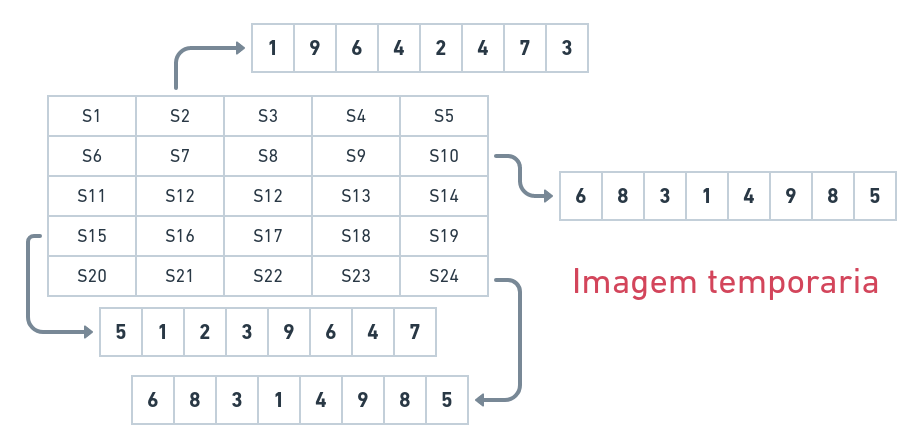
\includegraphics[width=\textwidth]{assets/solution.png}
    %\small{Incluir a imagem do exemplo de espaço de solução aqui}
\end{figure}

Algumas das implementações encontradas em bibliotecas de algoritmos populacionais de código aberto como \textit{PySwarms} utilizam internamente um sistema de representação de espaço de soluções de uma única dimensão, ou seja, uma lista simples, e utiliza uma função para transformar uma posição $[x,y]$ em um índice da lista. Essa implementação provavelmente foi escolhida por ser na maioria dos casos, mais rápida em comparação a uma abordagem de duas dimensões.\\
%% Fim do [Representações] %%
%% 2 ::: Desenvolvimento
%% 2.2 ::: Arquitetura
%% 2.2.2 ::: Espaço de Soluções
%% 2.2.2.2
%\subsubsection{Gráficos de análise}
\indent Como esse trabalho tem como foco uma exploração e implementação mais didática foi optado a utilização de uma representação em forma de uma matriz com duas dimensões, utilizando a biblioteca \textit{NumPy}. Essa abordagem em matriz de duas dimensões também facilita a geração de gráficos para representação visual, como, por exemplo, passar a matriz de soluções pela função de avaliação e assim obter um valor de \textit{fitness} para cada ponto do espaço de soluções, como é possível ver na 
\hyperref[fig:surfaceplot]{Figura \ref{fig:surfaceplot}} 
na qual os valores mais acima e mais escuros tem um valor de \textit{fitness} mais alto (ou seja, pior), e os valores mais abaixo e mais claros tem um \textit{fitness} mais baixo (ou seja, melhor).\hfill

\begin{figure}[ht]
    \centering
    \caption{Gráfico de Superfície representando um espaço de soluções}
    \label{fig:surfaceplot}
    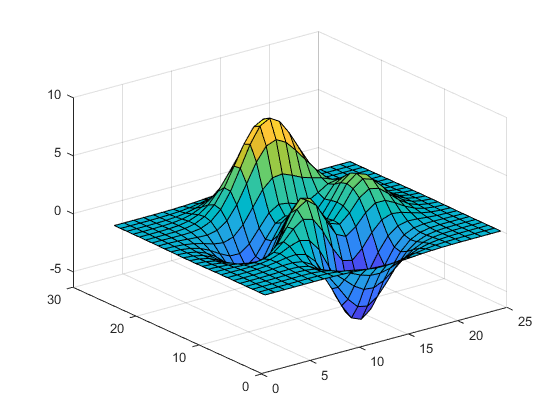
\includegraphics[width=\textwidth]{assets/surfaceplot.png}
    \small{* TODO - Adicionar valores no plot}
\end{figure}

Esses gráficos se mostraram uteis ao decorrer do desenvolvimento deste trabalho, servindo para validar detectar erros na função de inicialização do espaço de soluções.\\
%% Fim do [Gráficos de Analise] %%
%% 2 ::: Desenvolvimento
%% 2.2 ::: Arquitetura
%% 2.2.2 ::: Espaço de Soluções
%% 2.2.2.3
%\subsubsection{Influencia na Solução}
\indent A geração do espaço de soluções é muito importante para algoritmos como o PSO 
que funciona com base na movimentação conforme as médias de melhores posições, 
devido a isso, o PSO tente a ter problemas com convergência prematura em mínimos locais.\\
\indent Os mínimos locais são fenômenos onde dentro de uma parte do espaço de soluções existe um ponto que é melhor que a média dos pontos a sua volta, porém não é o melhor entre o todo o espaço de soluções, como é possível ver na \hyperref[fig:ex-minimolocal]{Figura \ref{fig:ex-minimolocal}}.\newline
\begin{figure}[ht]
    \centering
    \caption{Exemplo de um mínimo local}
    \label{fig:ex-minimolocal}
    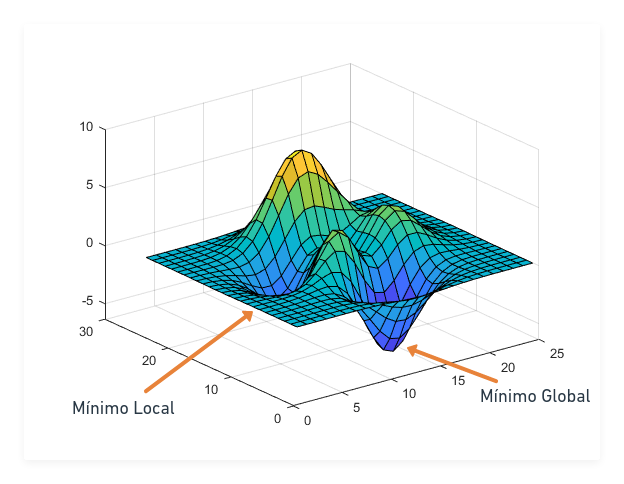
\includegraphics[width=\textwidth]{assets/minimo_local.png}
    %\small{}
\end{figure}
Por esse ponto se destacar entre seus vizinhos o algoritmo pode ficar preso nesta região, pois a média local sempre tende para o ponto onde está o mínimo local.\\
Como o PSO se baseia na média local e global, se houver mais de um mínimo local e quantidades equivalentes de partículas da população forem distribuídas para esses pontos, as partículas podem ficar presas já que as forças se balanceiam e o $gBest$ não muda mais.\\
%
\indent Já a convergência prematura acontece quando a um mínimo local e por coincidência a posição inicial da maioria das partículas da população tende a ser atraído para o mínimo local, logo a maioria da população para nesse ponto e o algoritmo termina em um estado como é mostrado na 
\hyperref[fig:convergencia-prematura]{Figura \ref{fig:convergencia-prematura}} 
ou seja, termina antes de encontrar uma solução tão boa quando seria possível.\\
\begin{figure}[ht]
    \centering
    \small{Incluir a convergência prematura aqui aqui}
    \caption{Demonstração de convergência prematura de uma população de partículas}
    \label{fig:convergencia-prematura}
\end{figure}
%% Fim do [Influencia na Solução] %%
%% 2 ::: Desenvolvimento
%% 2.2 ::: Arquitetura
%% 2.2.2 ::: Espaço de Soluções
%% 2.2.2.4
%\subsubsection{Implementação}
\indent Durante a implementação de um algoritmo para geração do espaço de soluções, foram percebidos diversos detalhes que influenciam fortemente na qualidade final do algoritmo. Nessa seção será analisado alguns desses pontos.\\
%\subsubsubsection{Inicialização}
\indent Um ponto importante percebido na implementação é como sera inicializado o \textit{array} onde será armazenado o espaço de soluções.\\
\indent O NumPy disponibiliza trés métodos de inicialização para um novo \textit{array} sem um valor de preenchimento, dos quais cada um demonstrou um problema diferente para a implementação. Dentre eles: 
\begin{itemize}
    \item \textit{numpy.zeros}: Ao inicializar o \textit{array} com todos os valores preenchidos com o valor "$0$", devido ao processo de embaralhamento das operações, o algoritmo pode acabar gerando resultados errôneos. Por não existir uma maquina $M_0$ algumas operações não eram consideradas no resultado, e devido à falta de algumas operações, a solução em questão tinha um valor de \textit{fitness} menor, o que tendia a fazer essa solução errônea a melhor.

    \item \textit{numpy.ones}: Ao inicializar o \textit{array} com todos os valores preenchidos com o valor "$1$", o algoritmo gerava soluções que tendiam a sobre carregar a máquina $M_1$ e assim os resultados finais tendiam a ter um valor de \textit{fitness} mais alto.

    \item \textit{numpy.empty}: Esse método de inicialização diferentemente dos outros, não defini nenhum valor para os registros da matriz, somente aloca um bloco de memória (semelhante ao \textit{malloc} da linguagem C), o que o torna mais rápido, porém ele traz o revés de possivelmente ter valores errados, pois por simplesmente alocar um bloco de memória, o \textit{array} pode ser inicializado com valores estranhos devido a lixo de memória.
\end{itemize}

\noindent Devido aos problemas citados acima, acaba sendo necessário de qualquer maneira percorrer todo o \textit{array} para setar valores. \newline 
Então foi optado por utilizar um método de preenchimento de valores aleatório, 
gerados pela função \textit{numpy.random.choice} que gera um \textit{array} de valores aleatórios seguindo uma distribuição uniforme, 
conforme demonstrado no Gráfico da \hyperref[fig:distrib-uniforme]{Figura \ref{fig:distrib-uniforme}}.

\begin{figure}[ht]
    \centering
    \small{Incluir o gráfico de distribuição aqui}
    \caption{Gráfico de distribuição de valores gerados pela função aleatória}
    \label{fig:distrib-uniforme}
\end{figure}

%
%% Inicialização do Array

Após as análises citadas acima foi feito uma modelagem e desenvolvido para esse trabalho o algoritmo de inicialização do espaço de soluções representado pelo 
\hyperref[fig:pseudocodigo-solutionspace]{Pseudo codigo \ref{fig:pseudocodigo-solutionspace}}. 
Além disso, a implementação real em Python está no apêndice x desse trabalho.\hfill

%% Todo - Apêndice
%% Todo - pseudo código
\begin{figure}[ht]
\centering
\small{Incluir o pseudo código de geração do espaço de soluções aqui}
\caption{Pseudo código da geração do espaço de soluções}
\label{fig:pseudocodigo-solutionspace}
\end{figure}
%
%% Fim do [Implementação] %%

%
%% Fim do [Espaço de Soluções] %%


    %% 2 ::: Desenvolvimento
    %% 2.2 ::: Arquitetura
    %% 2.2.3
    \subsection{Partícula}
        %% Interlúdio %%
            Por se tratar de um algoritmo populacional focado em partículas, por isso o nome \textit{Particle Swarm Optimization} que significa Otimização por Enxame de Partículas, a representação dessa entidade, assim como sua geração, controle e movimentação, se mostra um dos principais pilares do algoritmo. Devido a critérios de legibilidade e facilitação de futuros estudos nesse trabalho foi optado por criar uma estrutura de classe bem definida para essa representação e controle.
        %% Fim do [Interlúdio] %%


%% 2 ::: Desenvolvimento
%% 2.2 ::: Arquitetura
%% 2.2.3 ::: Partícula
%% 2.2.3.1
%\subsubsection{Implementação}
Nessa classe são guardados os valores de: posição, velocidade e $pBest$, além de outros dados utilizados para facilitar o gerenciamento como: valor da solução da sua atual posição, assim como seu valor de \textit{fitness} e o tamanho do espaço de soluções.\\
\indent Para fazer uma melhor movimentação foi optado por não usar uma variável de direção, mas sim uma variável que guarda a última posição onde a partícula esteve.\\
Além da armazenagem dos valores da partícula, a classe da Partícula também implementa algumas funções como:\\
Função \textbf{\textit{fill\_with\_random\_values}} que gera uma posição inicial e uma velocidade aleatória para a partícula.\\
Função \textbf{\textit{evaluate\_value}} que faz o cálculo do valor de \textit{fitness} da atual posição e a comparação do valor com o atual valor de $pBest$ e atualiza o $pBest$ caso o novo valor seja melhor.\\
Função \textbf{\textit{update\_position}} que faz a movimentação da partícula.\\
\noindent A implementação de toda a classe de partícula está disponível no apêndice x desse trabalho.\\
%% TODO - Apêndice
\indent Em implementações de código aberto como a já citada \textit{PySwarms}, também se utiliza uma representação de classe, porém sem nenhuma responsabilidade de cálculo de \textit{fitness}, atualização de posição ou de preenchimento de valores aleatórios na partícula.\\
%
%% Fim do [Representações] %%
%% 2 ::: Desenvolvimento
%% 2.2 ::: Arquitetura
%% 2.2.3 ::: Partícula
%% 2.2.3.3
%\subsubsection{Movimentação}
\indent A movimentação da partícula no espaço de soluções é o ponto mais importante dessa entidade. Pois, se não for feita da maneira certa pode fazer o algoritmo não desempenhar tão quanto o possível.\\
\indent Como a implementação do espaço de soluções foi feita utilizando uma representação matricial, o mecanismo de movimentação mais intuitivo seria uma movimentação por soma de inteiros.\\
\indent Aonde se tem uma direção e com base nessa direção se soma ou subtrai o valor de velocidade do eixo de movimento e assim se obtém uma nova posição, como mostrado no 
\hyperref[alg:mov-int-sum]{Pseudocódigo \ref{alg:mov-int-sum}}.\hfill

\begin{figure}[ht]
\centering
\small{Incluir o pseudo código de uma movimentação por soma de inteiros aqui}
\caption{Pseudocódigo de uma movimentação por soma de inteiros}
\label{alg:mov-int-sum}
\end{figure}

Ou seja, tendo uma posição $[15, 7]$ sendo $15$ o valor de $x$ e $7$ o valor de $y$,
uma velocidade $2$ e a direção do movimento ser \textit{CIMA}, a nova posição é obtida incrementado a velocidade ao valor de $y$ da posição, ou seja $[15, 7+2]$, então a nova posição seria $[15, 9]$, como pode ser visto na 
\hyperref[fig:movimentacao-int-sum]{Figura \ref{fig:movimentacao-int-sum}}.\hfill

\begin{figure}[ht]
\centering
\small{Incluir a demonstração de movimentação por soma de inteiros aqui}
\caption{Demonstração de movimentação por soma de inteiro}
\label{fig:movimentacao-int-sum}
\end{figure}

Essa abordagem funciona bem para uma movimentação simples em espaços 2D. Sendo inclusive muito utilizada no desenvolvimento de jogos com mapas baseados em ladrilhos (\textit{Tile-based} / \textit{Grid-based}).\\
\indent Porém, no caso do algoritmo PSO é necessário que ao calcular a nova posição, se considere a inércia e uma média entre o $pBest$ e o $gBest$, o que gera muitas vezes uma movimentação em ângulos mais específicos como representado na 
\hyperref[fig:angular-moviment-grid-based]{Figura \ref{fig:angular-moviment-grid-based}}
o que torna essa abordagem de soma de inteiros muito complexa e limitada para esse cenário.\hfill

\begin{figure}[ht]
\centering
\small{Incluir a imagem demonstrativa de movimentação com ângulos estranhos aqui}
\caption{Exemplo de movimentação com ângulos complexos}
\label{fig:angular-moviment-grid-based}
\end{figure}

%%%%

Então nesse trabalho foi desenvolvido um método de movimentação baseado em cálculos vetoriais que elimina esses problemas de movimentação além de facilitar a implementação de novos pontos de comparação (além do $pBest$ e $gBest$) para o cálculo da nova posição.\\
%\subsubsubsection{Movimentação Vetorial}
\indent Essa abordagem de movimentação é baseado no conceito de \textit{Produto Escalar} definido pela Álgebra Linear, e representa o produto interno padrão do espaço euclidiano sendo definido como uma operação binaria entre dois vetores.\\
\noindent Em um cenário aonde a posição da partícula é $position=[12,8]$ e $pBest=[10, 15]$, $gBest=[16,20]$ e $velocidade=[2,4]$.\\
\noindent Para encontrar a nova posição de uma partícula são utilizados:
\begin{itemize}
\item $\vec p$ Que representa o vetor entre a partícula e o $pBest$ 
(\hyperref[fig:vetor-p]{Figura \ref{fig:vetor-p}}).
\item $\vec g$ Que representa o vetor entre a partícula e o $gBest$ 
(\hyperref[fig:vetor-g]{Figura \ref{fig:vetor-g}}).
\item $\vec r$ Que representa o vetor final de movimento
(\hyperref[fig:vetor-r]{Figura \ref{fig:vetor-r}}).
\end{itemize}

\begin{figure}[!htb]
\begin{minipage}{\textwidth}

% 1º linha
\begin{minipage}{0.48\textwidth}
\centering
\caption{Vetor $\vec v$ de movimento}
\label{fig:vetor-v}
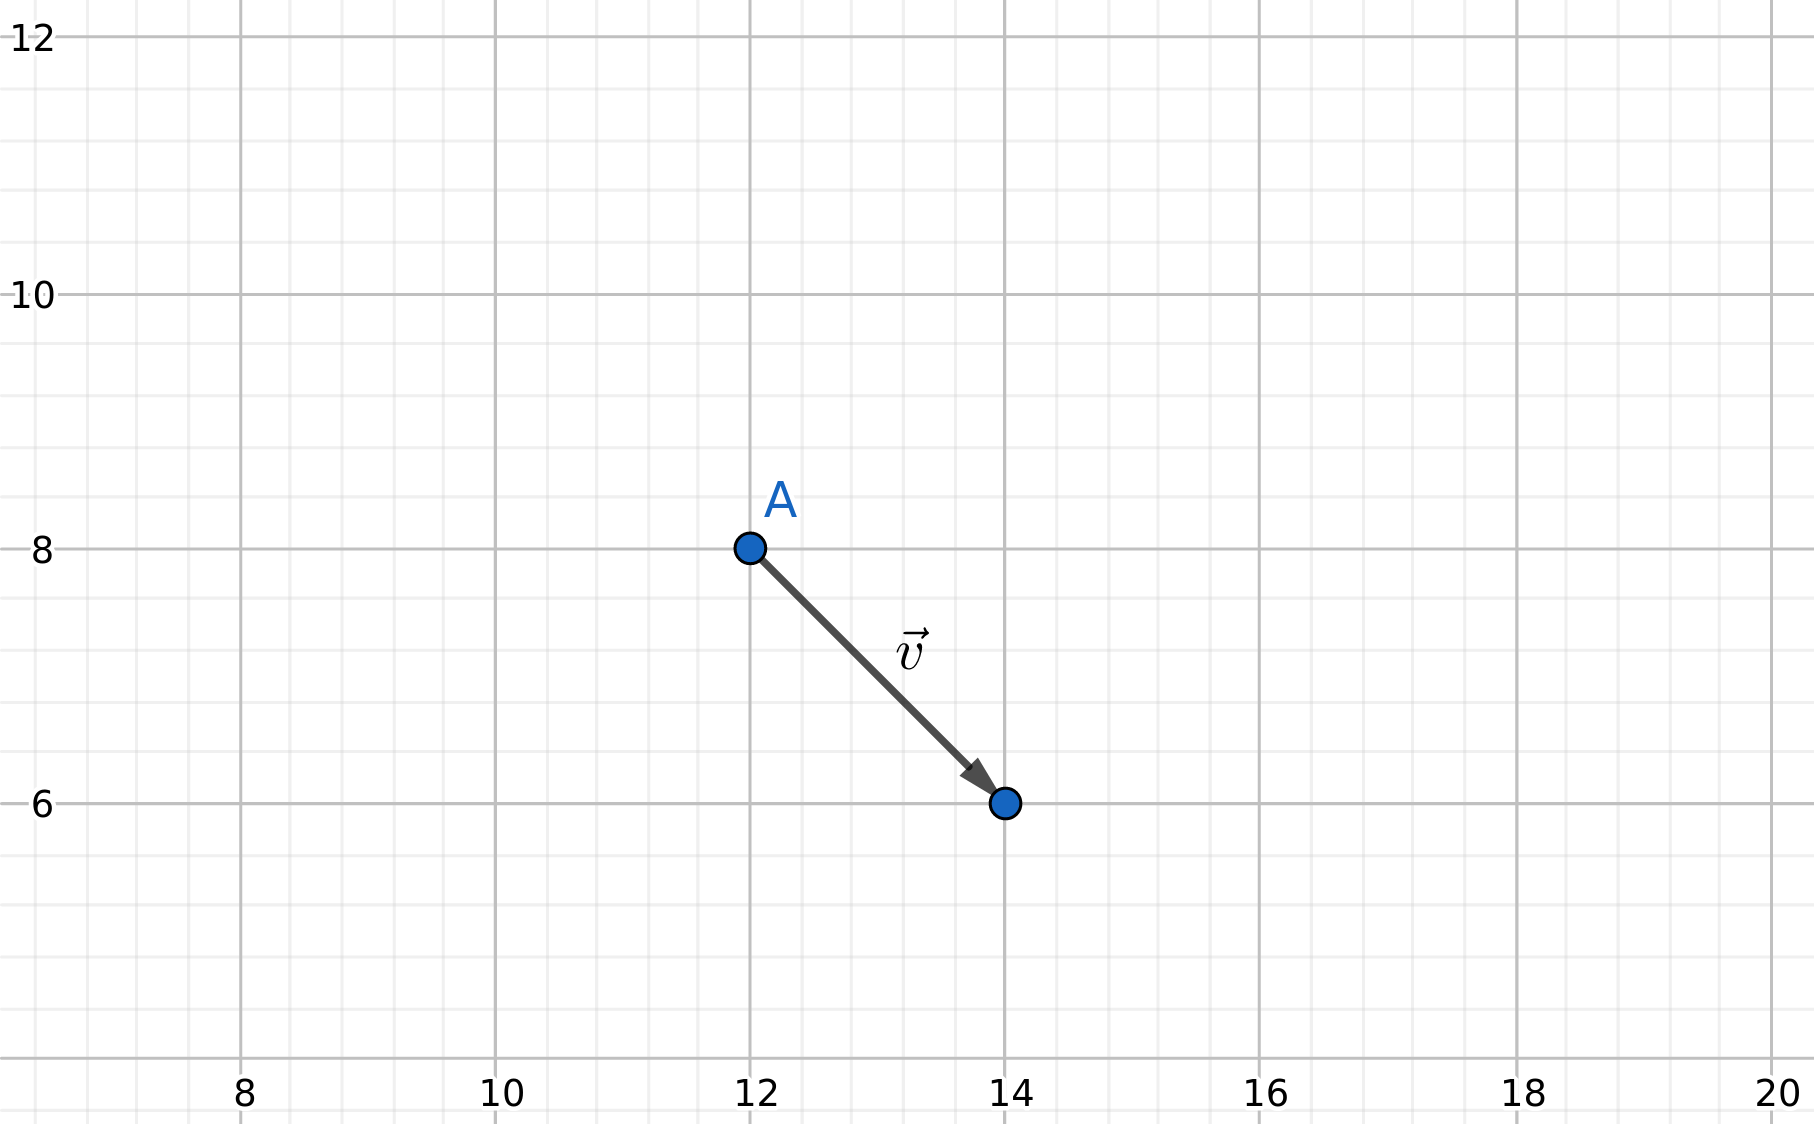
\includegraphics[width=.9\linewidth]{assets/vec1.png}
%\small{Incluir vetor v aqui}
\end{minipage}
\begin{minipage}{0.48\textwidth}
\centering
\caption{Vetor $\vec p$ de o $pBest$}
\label{fig:vetor-p}
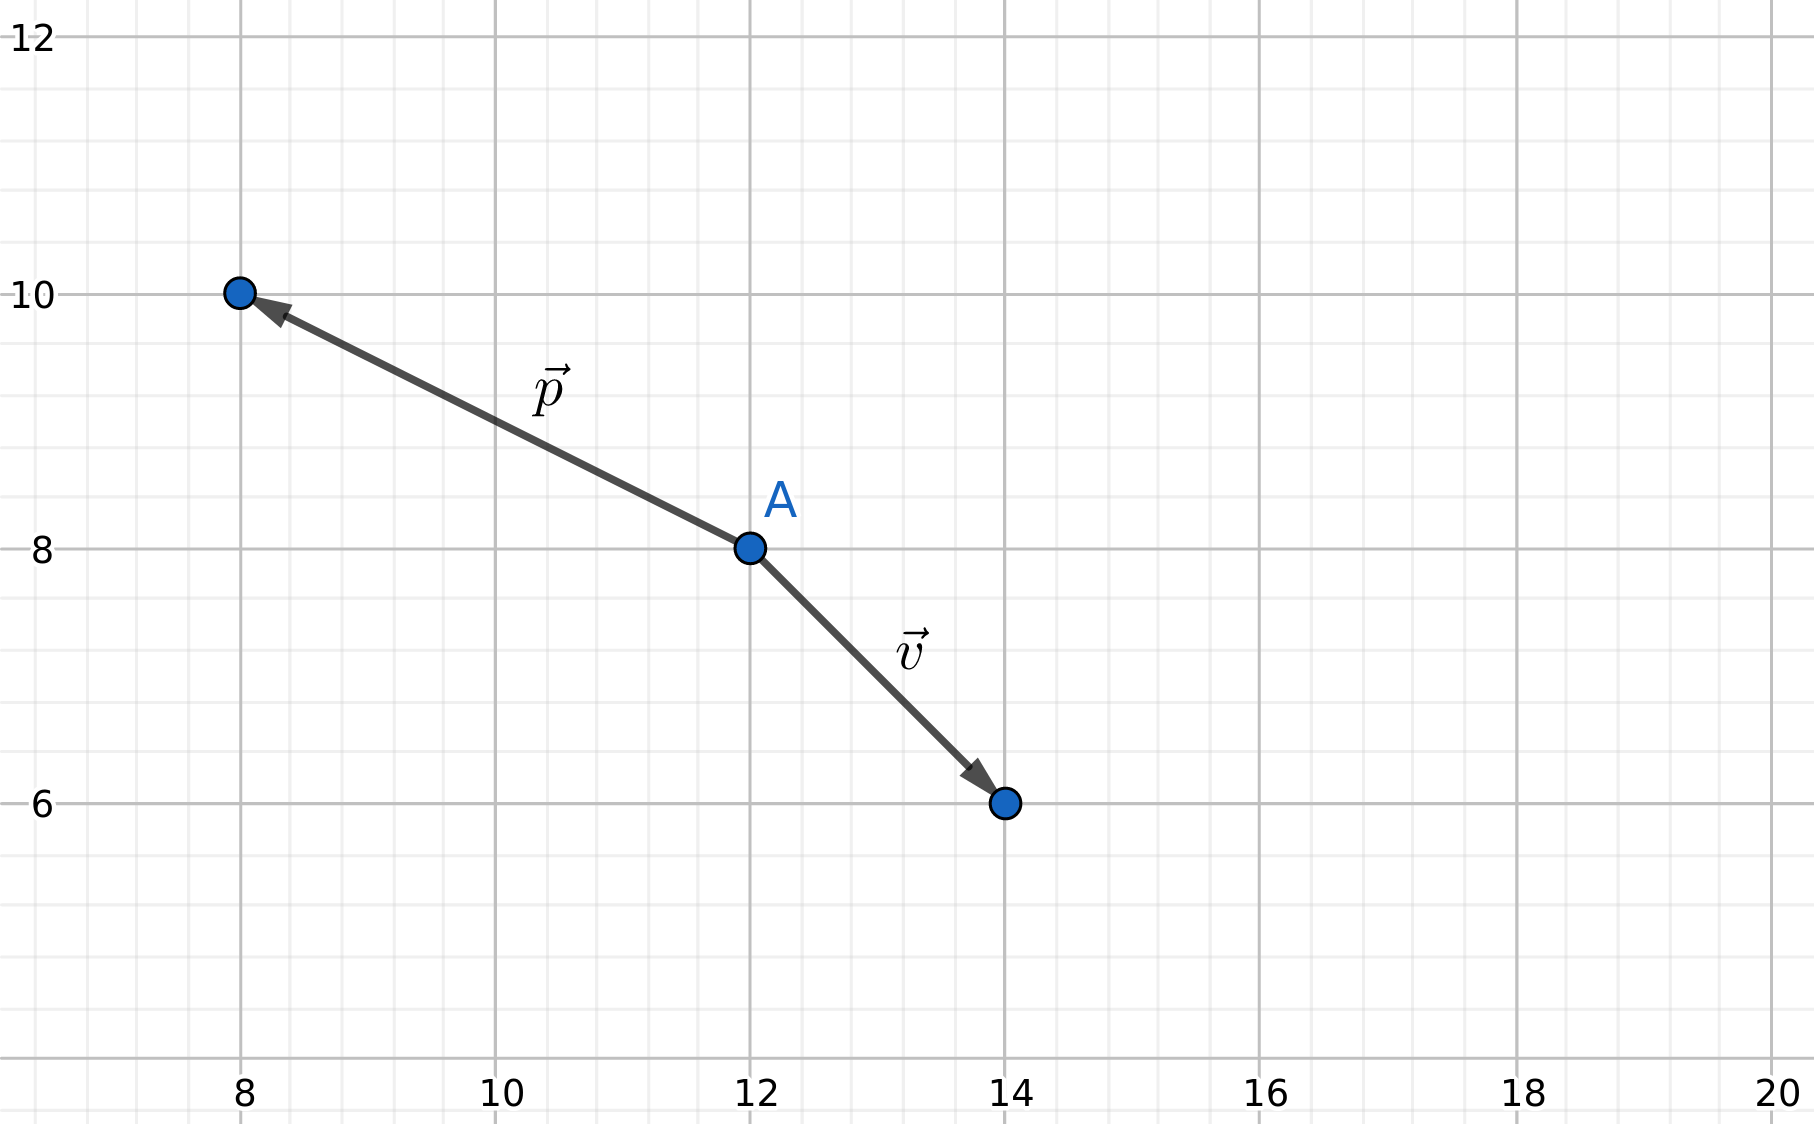
\includegraphics[width=.9\linewidth]{assets/vec2.png}
%\small{Incluir vetor p aqui}
\end{minipage}

% 2º linha
\begin{minipage}{0.48\textwidth}
\centering
\caption{Vetor $\vec g$ de o $gBest$}
\label{fig:vetor-g}
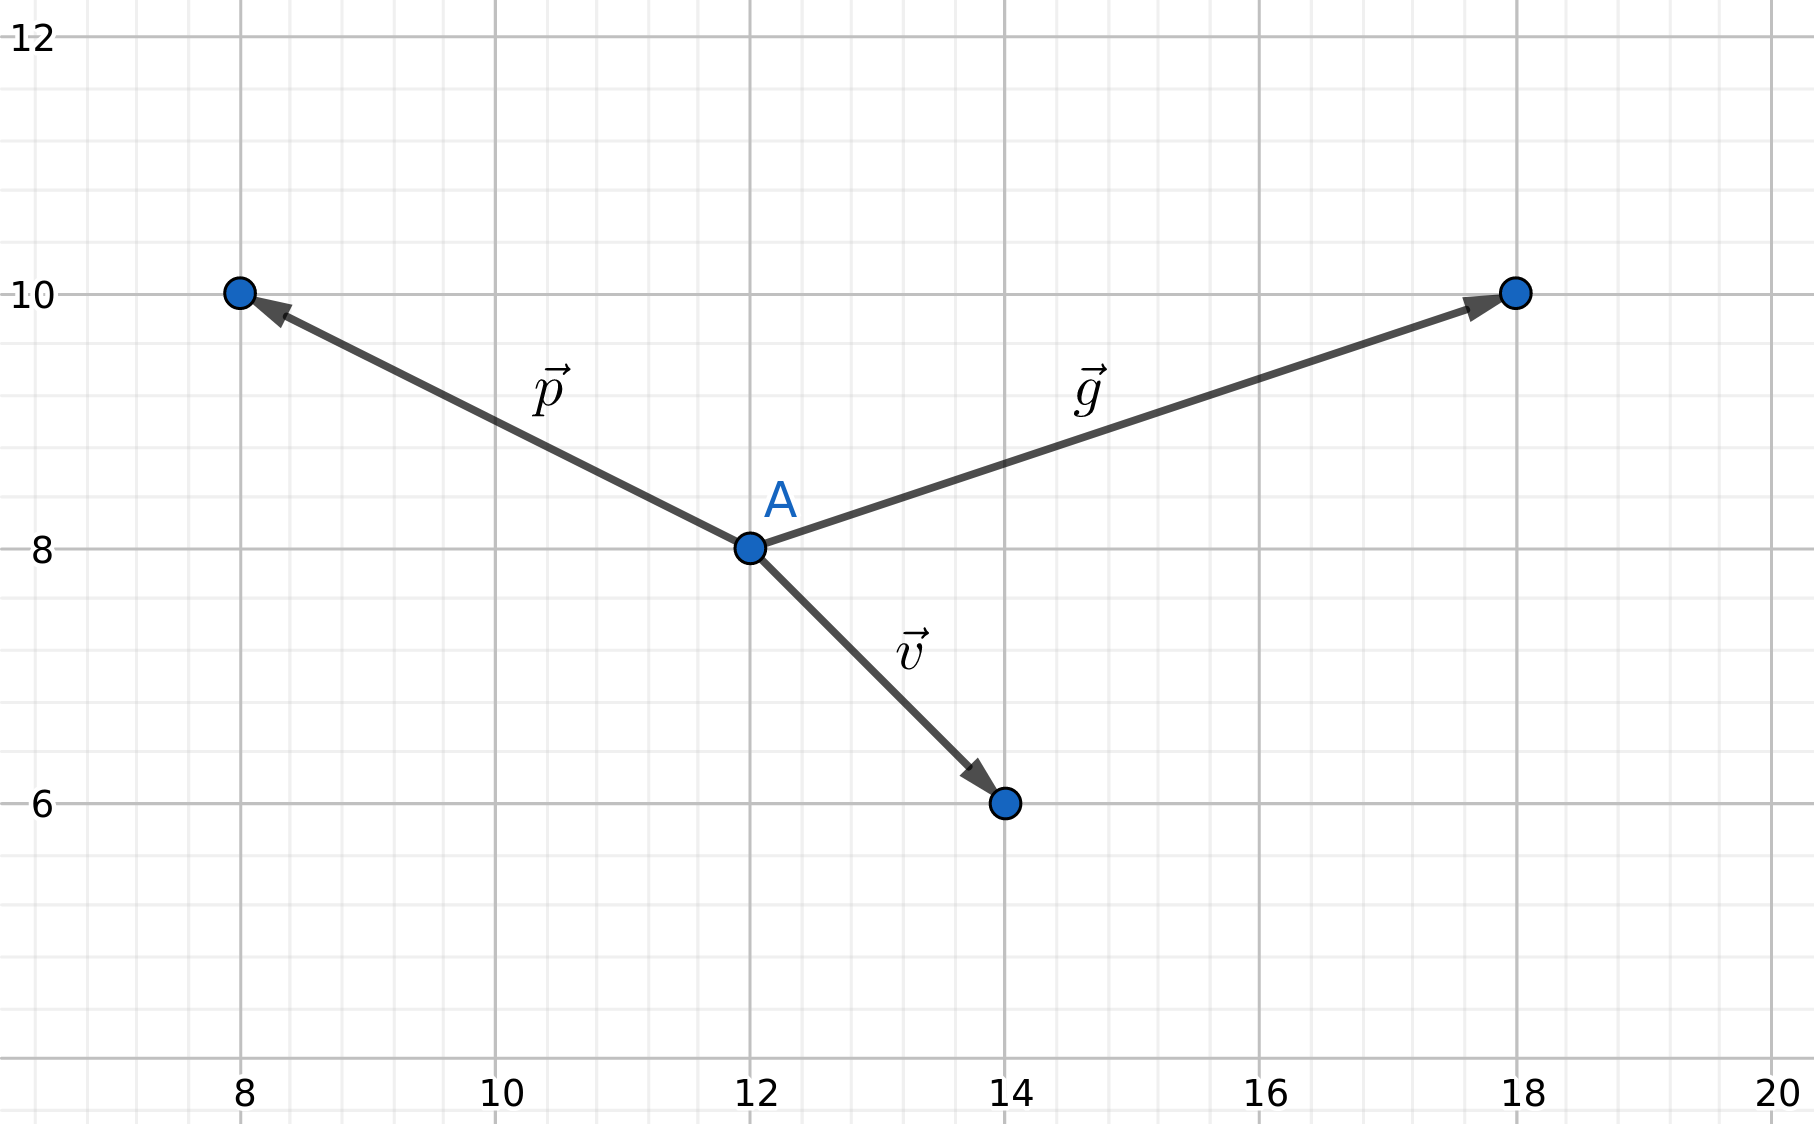
\includegraphics[width=.9\linewidth]{assets/vec3.png}
%\small{Incluir vetor g aqui}
\end{minipage}
\begin{minipage}{0.48\textwidth}
\centering
\caption{Vetor $\vec r$ de movimento final}
\label{fig:vetor-r}
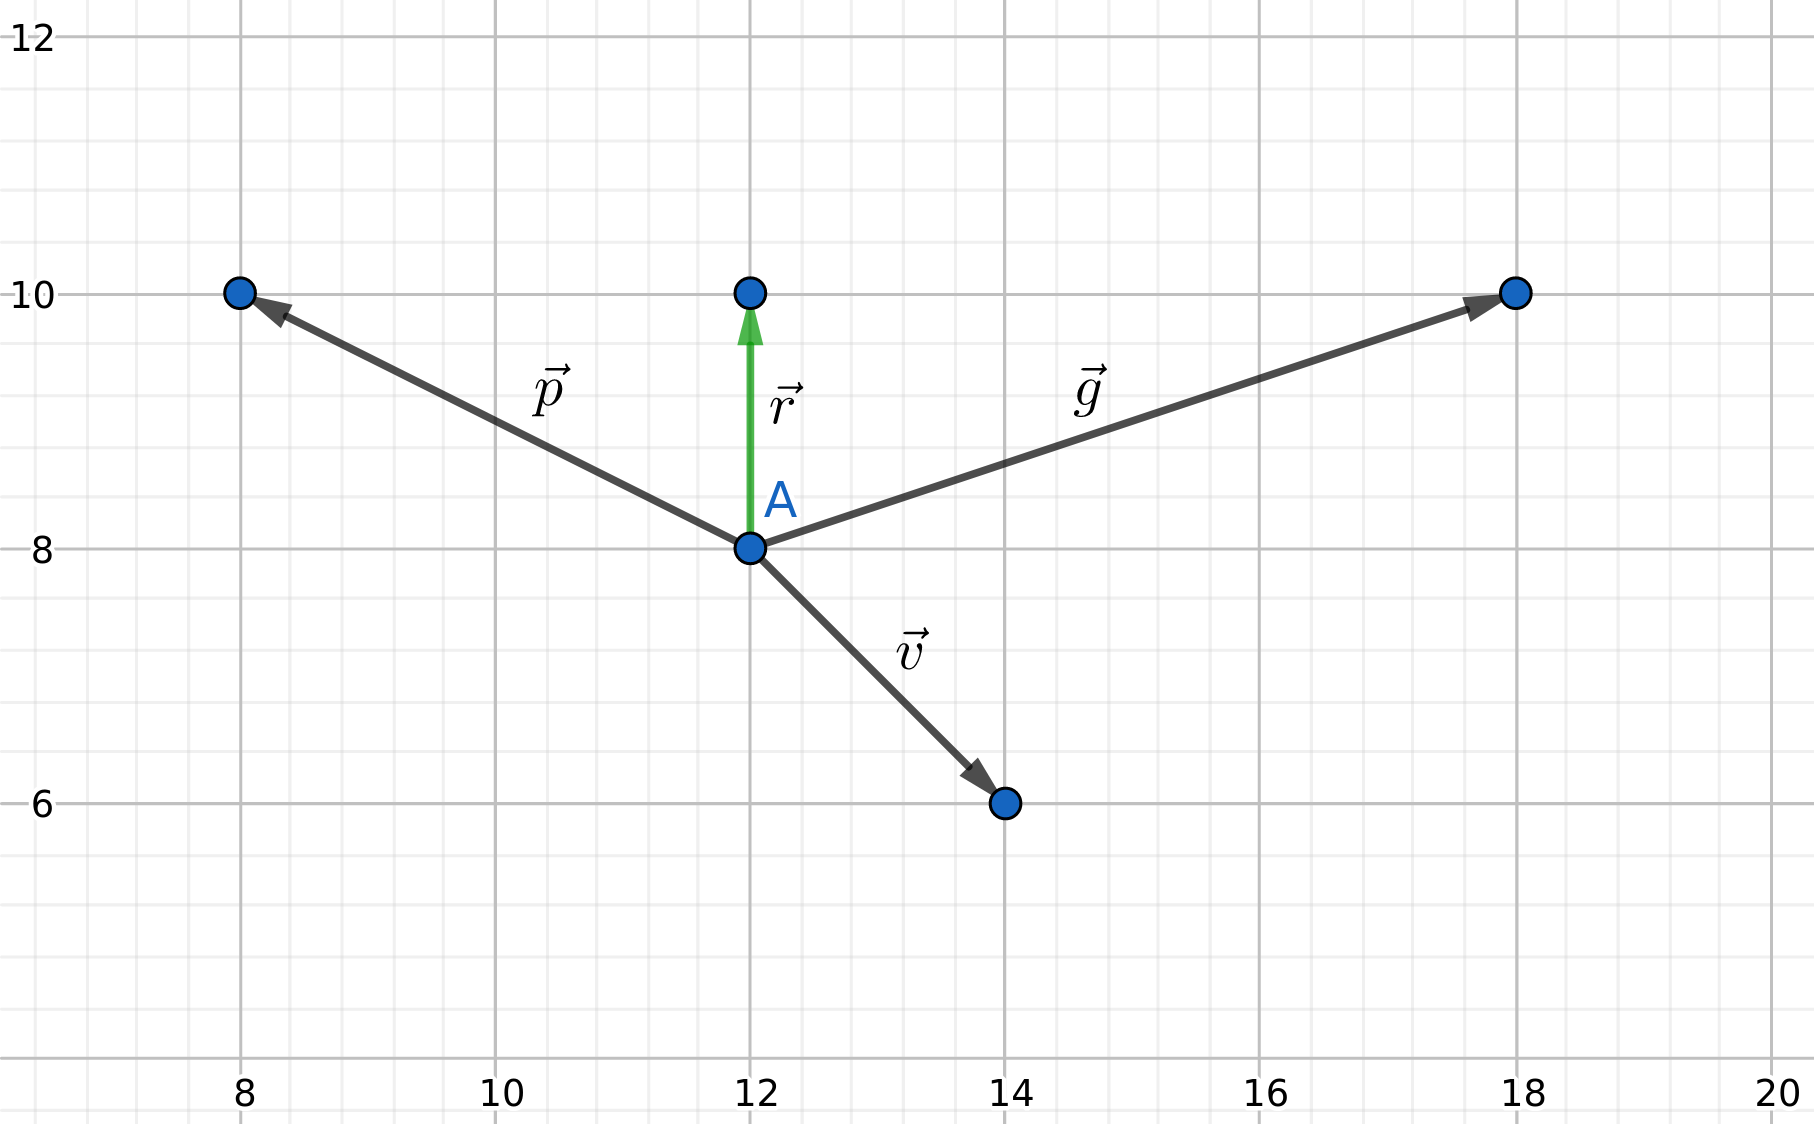
\includegraphics[width=.9\linewidth]{assets/vec4.png}
%\small{Incluir vetor w aqui}
\end{minipage}

\end{minipage}
\end{figure}

\noindent A nova posição da partícula é dada pela 
\hyperref[eq:movimentacao-vec]{Equação \ref{eq:movimentacao-vec}}
.
%
\begin{equation} 
    \label{eq:movimentacao-vec}
    \vec r = ((\vec g + \vec p) / 2) + \vec v
\end{equation}

\noindent Então temos o vetor $\vec r$ resultante, então a nova posição da partícula é $[12,10]$.

No código Python essa implementação é feita de maneira levemente diferente por características da linguagem. Para realizar os cálculos vetoriais foi utilizado a biblioteca \textit{Numpy}.\\
\indent Para isso primeiro é calculo um vetor médio entre $pBest$ e $gBest$, e o vetor $\vec w$ representando a inércia.\\
\indent Então a posição atual da partícula é deduzido do valor médio entre $pBest$ e $gBest$, isso é feito para que calcular o vetor como se a posição atual da partícula fosse o ponto $[0,0]$ do mapa.\\
Então somado com o vetor de inércia divido por um valor de significância para a inércia (Definido pelos parâmetros de configuração do algoritmo).\\
%
\indent No \hyperref[alg:mov-part]{Pseudocódigo \ref{alg:mov-part}} é possível ver a representação dessa função de cálculo, e a implementação desse método está disponível no apêndice x.
%% TODO - apêndice
\begin{algorithm}
    \caption{Pseudocódigo de movimentação de particula}\label{alg:mov-part}
\begin{algorithmic}
\State vetor de inercia $\gets$ (posicao inicial $*$ velocidade)
\State melhor media $\gets$ ($pBest$ + $gBest$) / 2
\State vetor final $\gets$ (melhor media + posição inicial) / 2
\end{algorithmic}
\end{algorithm}

%
%% Fim do [Movimentação Vetorial] %%


%
%% Fim do [Movimentação] %%

%
%% Fim do [Partícula] %%


%% 2 ::: Desenvolvimento
%% 2.2 ::: Arquitetura
%% 2.2.4
\subsection{População}
Pelo algoritmo PSO ser um algoritmo baseado em inteligência populacional, ele é muito influenciado pela geração da população inicial, mesmo nos algoritmos com variações aonde existem mutações e consequentemente evolução dos indivíduos da população, as características como inercia, velocidade, direção e posição desses indivíduos da população inicial são de grande importância.\\
\indent Os parâmetros como o tamanho da população são definidos nas configurações do algoritmo. Todas as funções utilizadas na geração dos indivíduos seguem o padrão de distribuição uniforme.\\
\indent A posição inicial da partícula é dada por dois números aleatórios entre $1$ e o limite do espaço de soluções $- 1$.\\
\indent A última posição da partícula é obtida através de um sorteio de chances iguais que pode ou subtraindo, ou adicionar o valor $1$ na posição inicial gerada anteriormente. Caso seja subtraído $1$ a direção do movimento é para frente, caso seja subtraído $1$ a direção do movimento é para trás.\\
\indent A velocidade é dada por um valor aleatório entre $0.1$ e $0.2$.\\
\indent Assim, como valores iniciais seguindo uma distribuição uniforme é observado uma geração de população inicial bem distribuída, dificultando o acontecimento de convergência prematura.

Sendo assim, todas as variações do algoritmo PSO implementadas nesse trabalho utilizam a mesma função geradora de população inicial, representada pelo código no apêndice x. %%TODO apendice  
\noindent Garantindo assim um ponto de comparação mais justo entre os algoritmos.
%% 2 ::: Desenvolvimento
%% 2.2 ::: Arquitetura
%% 2.2.5
\subsection{Algoritmos}
%%
A execução dos algoritmos é chamada pela classe principal da modelagem do problema, sendo responsavel por fazer a execução e controle dos dados de analise.\\
Na classe do PSO estão as funções da condição de parada, movimento e \textit{evaluete} do \textit{fitness} da particula. A implementação esta disponivel no apendice x.\\ %todo apendice
%
%
Como criterio de parada para o algoritmo foi utilizado o fator de atualização do $gBest$. Quando a ultima atualização do $gBest$ for a mais rodadas do que metade da quantidade de particulas, o algoritmo termina e o resultado é o $gBest$ atual.\\
%%
\indent O que diferencia as abordagens analisadas nesse trabalho são as heuristicas de movimentação das particulas.\\
A movimentação basica de uma particula do PSO é definido pela
\hyperref[eq:movimentacao-particula]{Equação \ref{eq:movimentacao-particula}}
.
%
\begin{equation} 
    \label{eq:movimentacao-particula}
    \vec v_1(t+1)= \vec v_i(t) + a_1 r_1 (pBest - \vec x_i(t)) + a_2 r_2 (gBest - \vec x_i(t))
\end{equation}
%
Como foi observado nos testes a variavel aleatoria é importande para que as particulas não entrem em um estado de equilibrio e não se movam mais, como demonstrado na \hyperref[fig:equelibrio-particulas]{Figura \ref{fig:equelibrio-particulas}}.
\begin{figure}[ht]
    \centering
    \small{Incluir a aaaaaaaaaaaaaaaaaaaaaaaa aqui}
    \caption{Equilibrio nas forças de movimentação de particula}
    \label{fig:equelibrio-particulas}
\end{figure}

Com esse elemento aleatorio a movimentaçãos e torna mais caotica e evita o fim prematuro do algoritmo, como representado na \hyperref[fig:rand-particulas]{Figura \ref{fig:rand-particulas}}.
\begin{figure}[ht]
    \centering
    \small{Incluir a aaaaaaaaaaaaaaaaaaaaaaaa aqui}
    \caption{Equilibrio nas forças de movimentação de particula}
    \label{fig:rand-particulas}
\end{figure}

Esse impacto na movimentação inspirou uma abordagem que considera o nivel de atualizações de $gBest$ e assim adiciona mais um fator aleatorio no calculo. como é representado no 
\hyperref[alg:mov-dinamic]{Pseudocódigo \ref{alg:mov-dinamic}}.
\begin{algorithm}
    \caption{Pseudocódigo de movimentação com componente dinamico}\label{alg:mov-dinamic}
\begin{algorithmic}

\State vetor de inercia $\gets$ (posicao inicial $*$ velocidade)
\State melhor media $\gets$ (($pBest$ + $gBest$) / 2)
\State vetor final $\gets$ ((melhor media + posição inicial) / 2)

\If{trocas de $gBest$ é menor que (tamanho da populacao / $10$)}
    \State vetor final $\gets$ vetor de movimento $+$ $0.1$ $*$ (inercia$*$random($0.1$, $0.9$) )
\Else
    \State vetor final $\gets$ vetor de movimento $+$ $0.1$ $*$ random($0.1$, $0.9$) 
\EndIf    
\end{algorithmic}
\end{algorithm}

%% Fim do [Algoritmos] %%
%% Fim do [Arquitetura] %%
%% 2 ::: Desenvolvimento
%% 2.3
\section{Execuções}
Pela natureza variável do ambiente em nuvem cada teste de algoritmo foi executado 30 vezes para obter uma média dos tempos de execução.\hfill\vspace{\onelineskip}

Como foi descrito anteriormente, de modo a assegurar uma análise mais detalhada, os dados gerados pelos algoritmos foram salvos em aquivo texto para análise detalhada.\hfill\vspace{\onelineskip}

Os dados salvos são:
\begin{itemize}
\item População inicial.
\item Espaço de soluções.
\item Números de rodadas do algoritmo.
\item Histórico da variável $gBest$.
\item Histórico da variável $pBest$.
\item Histórico da posição das partículas.
\item Soluções encontradas.
\end{itemize}

(Dados a completar...)
% 
%% Fim do [Execuções] %%


%% 2 ::: Desenvolvimento
%% 2.4
\section{Critérios de Avaliação}
A partir das médias estatísticas das execuções, são utilizados como critérios de avaliação do algoritmo: \hfill
\begin{itemize}
\item Tempo total de execução do algoritmo.
\item \textit{Fitness} final.
\end{itemize}

\noindent E são parâmetros de análise:\hfill
\begin{itemize}
\item Taxa de mudança da variável $gBest$ ao longo da execução.
\item Quantidade de rodadas necessárias para atingir o critério de parada.
\item Taxa de mudanças de $pBest$ por rodada.
\item Histórico de movimentação das partículas.
\end{itemize}

Além desses critérios também é possível observar os dados e tirar outras conclusões sobre o comportamento do algoritmo.\hfill

%
%% Fim do [Critérios de Avaliação] %%


%% 2 ::: Desenvolvimento
%% 2.5
\section{Resultados}
(Dados a completar...)
%
%% Fim do [Resultados] %%

\chapter{Conclusão}
%\lipsum[1]



\cleardoublepage
%%%%% Fim dos Elementos Textuais %%%%%

%%%%%%%%%%%%%%%%%%%%%%%%%%%%%%%%%%%%%%%%%%%%%%%%%%%%%%%%%%%%%%%%%%%%%%%%%%%%%%%%%%%%%%%%%%%
%%%%%%%%%%%%%%%%%%%%%%%%%%%%%%%%%%%%%%%%%%%%%%%%%%%%%%%%%%%%%%%%%%%%%%%%%%%%%%%%%%%%%%%%%%%
%%%%%%%%%%%%%%%%%%%%%%%%%%%%%%%%%%%%%%%%%%%%%%%%%%%%%%%%%%%%%%%%%%%%%%%%%%%%%%%%%%%%%%%%%%%

%%%%% Elementos pós-textuais %%%%%
\postextual

\bibliography{assets/references.bib}{}

\chapter{Apêndices}

\appendix

%\section{Função Geradora de População Inicial}
\label{apd:fun-gen-init-pop}
    (Codigoooo...)
%%%%

%\section{Classe PSO}
\label{apd:pso-class}
%%%%

%\section{Classe Particula}
\label{apd:particule-class}
%%%%

%\section{Classe de Decoder}
\label{apd:decode-class}
    (Codigoooo...)
%%%%

%\section{Classe de Encoder}
\label{apd:encode-class}
    (Codigoooo...)
%%%%

\label{apd:problem-instances}

\section{Instancias do Problema A}
\label{apd:problem-instance-a}
    (Tabelaaaa...)
%%%%
\section{Instancias do Problema B}
\label{apd:problem-instance-b}
    (Tabelaaaa...)
%%%%
\section{Instancias do Problema C}
\label{apd:problem-instance-c}
    (Tabelaaaa...)
%%%%
\section{Instancias do Problema D}
\label{apd:problem-instance-d}
    (Tabelaaaa...)
%%%%




%%%%% Fim dos Elementos pós-textuais %%%%%
\end{document}